% This is a LaTeX thesis template for Monash University.
% to be used with Rmarkdown
% This template was produced by Rob Hyndman
% Version: 6 September 2016

\documentclass{monashthesis}

%%%%%%%%%%%%%%%%%%%%%%%%%%%%%%%%%%%%%%%%%%%%%%%%%%%%%%%%%%%%%%%
% Add any LaTeX packages and other preamble here if required
%%%%%%%%%%%%%%%%%%%%%%%%%%%%%%%%%%%%%%%%%%%%%%%%%%%%%%%%%%%%%%%

\author{Stephanie Rose Kobakian}
\title{New algorithms for effectively visualising Australian spatio-temporal disease data.}
\degrees{B.Comm. and B.Eco., Monash University}
\def\degreetitle{Master of Philosophy (Statistics)}
% Add subject and keywords below
\hypersetup{
     %pdfsubject={The Subject},
     %pdfkeywords={Some Keywords},
     pdfauthor={Stephanie Rose Kobakian},
     pdftitle={New algorithms for effectively visualising Australian spatio-temporal disease data.},
     pdfproducer={Bookdown with LaTeX}
}


\bibliography{thesisrefs}

\begin{document}

\pagenumbering{roman}

\titlepage

{\setstretch{1.2}\sf\tighttoc\doublespacing}

\hypertarget{copyright-notice}{%
\chapter*{Copyright notice}\label{copyright-notice}}
\addcontentsline{toc}{chapter}{Copyright notice}

\textcopyright { } \authorname~(\number\the\year).

I certify that I have made all reasonable efforts to secure copyright permissions for third-party content included in this thesis and have not knowingly added copyright content to my work without the owner's permission.

\newpage

\hypertarget{keywords}{%
\chapter*{Keywords}\label{keywords}}
\addcontentsline{toc}{chapter}{Keywords}

Keywords:
cartogram; choropleth; geospatial statistics; maps; statistics; tile maps; visual inference

\hypertarget{abstract}{%
\chapter*{Abstract}\label{abstract}}
\addcontentsline{toc}{chapter}{Abstract}

The goal of many spatial visualisations is to gain a broad perspective of the values of statistics over the Australian population. However, the use of most mapping techniques can mislead, as the use of geographical areas unequally presents the spatial distribution of a dataset. The Australian population has congregated in the capital cities and significant cities in each state. This pattern has resulted in very dense population centres and sparsely populated rural areas. The relationship between the Australian population and the geographic area they live in results in a heterogeneous distribution of the map space.

As part of this thesis, an algorithm is presented which will take geospatial areas in the form of polygons and create an alternative graphical display of a spatial distribution. This algorithm takes a set of polygons and creates a map of tessellated hexagons, representing a single geographical area with a single hexagon. It arranges them to replicate spatial relationships of geographic areas in each city. The hexagon tile map visualisation produced by the algorithm is contrasted with the traditional choropleth map.
The package \texttt{sugarbag} \autocite{sugarbag} implements the algorithm for the statistical software \texttt{R} \autocite{R}.

Using animations will allow us to control how people transform a recognisable map of Australia, or the cities within, into a more reliable map for inference. Animation is gaining popularity as access to computing power is increasing the amount of applications.

\newpage

\hypertarget{list-of-figures}{%
\chapter*{List of Figures}\label{list-of-figures}}
\addcontentsline{toc}{chapter}{List of Figures}

\begin{tabular}{lrl>{\raggedleft\arraybackslash}p{20em}}
\toprule
Chapter & Figure & Caption & Page\\
\midrule
2 & 1 & A selection of choropleth cancer maps from online atlases that are publicly available. & 12\\
2 & 2 & Common alternatives to maps, showing the same information for the United States of America. & 20\\
2 & 3 & Two alternative displays, tile map (left) and geofaceted map (right), showing state age-adjusted rate of incidence for lung and bronchus in the USA. & 24\\
2 & 4 & Cartograms showing melanoma incidence in Australia. & 26\\
2 & 5 & Interactive controls of displays in publicly available choropleth cancer maps & 30\\
\addlinespace
2 & 6 & Two examples of advanced interactivity (and animation) in publicly available choropleth cancer maps. & 32\\
3 & 1 & Grid points to create a tilegram. & 44\\
3 & 2 & All possible hexagon locations from the initial grid are shown with blue outlines. & 45\\
3 & 3 & Filter for grid points within a square, then circular, distance for those closest to the centroid. & 47\\
3 & 4 & A complete hexagon tile map of Tasmania & 48\\
\addlinespace
3 & 5 & The Australian Cancer Atlas data has determined the colour of each Statistical Area of Australian at Level 2 & 48\\
3 & 6 & A choropleth map of the Statistical Areas of Australia at Level 2. & 51\\
3 & 7 & A hexagon tile map of the Statistical Areas of Australia at Level 2. & 52\\
4 & 1 & A choropleth map of the smoothed average of liver cancer diagnoses for Australian males. & 60\\
4 & 2 & A hexagon tile map of the smoothed average of liver cancer diagnoses for Australian males. & 60\\
\addlinespace
4 & 3 & This lineup of twelve hexagon tile map displays contains one map with a real population related structure. & 61\\
4 & 4 & The experimental design used in the visual inference study. & 62\\
4 & 5 & The detection rates achieved by participants are contrasted when viewing the four replicates of the three trend models & 64\\
4 & 6 & The distribution of the time taken (seconds) to submit a response for each combination of trend, whether the data plot was detected, and type of display, shown using horizontally jittered dotplots. & 65\\
4 & 7 & The amount of times each level of certainty was chosen by participants when viewing hexagon tile map or choropleth displays. & 66\\
\bottomrule
\end{tabular}

\hypertarget{list-of-tables}{%
\chapter*{List of Tables}\label{list-of-tables}}
\addcontentsline{toc}{chapter}{List of Tables}

\begin{tabular}{lll>{\raggedleft\arraybackslash}p{20em}}
\toprule
Chapter & Table & Caption & Page\\
\midrule
2 & 1 & A selection of choropleth cancer maps from online atlases. & 10\\
2 & 2 & Common measures for reporting cancer information. & 13\\
2 & 3 & Maps used to present statistics for the United States of America. & 18\\
2 & 4 & Summary of features and constraints of common mapping methods used to display
cancer statistics. & 26\\
4 & I (1) & The mean and standard deviation of the rate of detection for each trend model, calculated for the choropleth and hexagon tile map displays. & 64\\
\addlinespace
4 & II (2) & The model output for the generalised linear mixed effect model for detection rate. & 65\\
4 & III (3) & The amount of participants that selected each reason for their choice of plot when looking at each trend model shown in Choropleth and Hexagon Tile maps. & 66\\
\bottomrule
\end{tabular}

\hypertarget{list-of-publications}{%
\chapter*{List of Publications}\label{list-of-publications}}
\addcontentsline{toc}{chapter}{List of Publications}

\begin{enumerate}
\def\labelenumi{\arabic{enumi}.}
\tightlist
\item
  The literature review exploring current practice for visualising spatial data in Chapter \ref{ch:literature} has been submitted to the journal \emph{Annals of Cancer Epidemiology} for publication.
\end{enumerate}

Kobakian S. and Cook, D. and Roberts, J. (2019). Cancer Applications of Choropleth Maps, and the Potential of Cartograms and Alternative Map Displays. Manuscript submitted for publication.

\begin{enumerate}
\def\labelenumi{\arabic{enumi}.}
\setcounter{enumi}{1}
\tightlist
\item
  The details of the algorithm documented in Chapter \ref{ch:algorithm} have been submitted to the \emph{Journal of Statistical Software}.
\end{enumerate}

Kobakian S. and Cook, D. (2020). An Algorithm For Spatial Mapping Using a Hexagon Tile Map, With Application to Australian Maps. Manuscript submitted for publication.

\begin{enumerate}
\def\labelenumi{\arabic{enumi}.}
\setcounter{enumi}{2}
\tightlist
\item
  The details of the visual inference testing is documented in Chapter \ref{ch:experiment} has been submitted to the \emph{IEEE Transactions of Visualisation and Computer Graphics} under the title ``Comparing the Effectiveness of the Choropleth Map with a Hexagon Tile Map for Communicating Cancer''
\end{enumerate}

Kobakian S. and Cook, D. (2020). Comparing the Effectiveness of the Choropleth Map
with a Hexagon Tile Map for Communicating Cancer Manuscript submitted for publication.

\begin{enumerate}
\def\labelenumi{\arabic{enumi}.}
\setcounter{enumi}{3}
\tightlist
\item
  The code for the algorithm documented in Chapter \ref{ch:algorithm} is currently hosted on \emph{CRAN} as the package sugarbag.
\end{enumerate}

Kobakian, S. and Cook, D. (2019). sugarbag: Create Tessellated Hexagon Maps. \url{https://srkobakian.github.io/sugarbag/}, \url{https://github.com/srkobakian/sugarbag}.

\clearpage\pagenumbering{arabic}\setcounter{page}{0}

\hypertarget{declaration}{%
\chapter*{Declaration}\label{declaration}}
\addcontentsline{toc}{chapter}{Declaration}

I hereby declare that this thesis contains no material which has been accepted for the award of any other degree or diploma at any university or equivalent institution and that, to the best of my knowledge and belief, this thesis contains no material previously published or written by another person, except where due reference is made in the text of the thesis.

This thesis includes three original papers submitted to peer reviewed journals. The core theme of the thesis is spatial visualisations. The ideas, development and writing up of all the papers in the thesis were the principal responsibility of myself, the student, working within the Faculty of Science and Engineering under the supervision of Distinguished Professor Kerrie Mengersen and Dr.~Earl Duncan. It was also created under the supervision of the external supervisor Professor Dianne Cook.

The papers in Chapters 2, 3, and 4 have been individually formatted for journal submission however, I have renumbered the pages of the submitted papers for cohesion across this thesis.

\hypertarget{acknowledgements}{%
\chapter*{Acknowledgements}\label{acknowledgements}}
\addcontentsline{toc}{chapter}{Acknowledgements}

This thesis would not be possible without the opportunity provided by Queensland University of Technology, Cancer Council Queensland and the ARC Centre of Excellence for Mathematical \& Statistical Frontiers.

I would like to acknowledge my supervisors for their tireless work in directing, encouraging and supporting this work.

Professor Kerrie Mengersen (Professor of Statistics, Science and Engineering Faculty, QUT) provided the opportunity to study at Queensland University of Technology, organising and supervising this project.

Dr Earl Duncan (Research Associate at ARC Centre of Excellence for Mathematical \& Statistical Frontiers, QUT) provided time and effort for to discussion, editing and commenting throughout this degree.

Professor Dianne Cook (Professor, Department of Econometrics and Business Statistics, Monash University) provided constant support, encouragement and recommendations throughout this degree.
Working closely with Prof.. Di Cook enabled the rapid development of my research and writing skills.

\hypertarget{literature-review}{%
\section{Literature review}\label{literature-review}}

We would like to acknowledge Dr Susanna Cramb (Spatial Modeller, Cancer Council Queensland) and Dr Peter Baade (Senior Research Fellow, Cancer Council Queensland) for providing the opportunity and time to discuss alternative map solutions for presentation in the Australian Cancer Atlas.
It was in the development of this online cancer atlas that methods for disease map displays, and visual communication strategies were explored.

\hypertarget{visual-inference-study}{%
\section{Visual inference study}\label{visual-inference-study}}

Stephanie would like to thank Mitchell O'Hara-Wild was a co-developer of the taipan \autocite{taipan} R package for the web app constructed to collect participant evaluations of lineups.

We are thankful for the NUMBATs (Non-Uniform Monash Business Analytics Team) for participating in the pilot study that helped to assess the experimental design and determine an appropriate sample size for the study.

\hypertarget{r-packages}{%
\section{R packages}\label{r-packages}}

Several \texttt{R} \autocite{R} packages were used to produce this thesis:

\begin{itemize}
\tightlist
\item
  \texttt{absmapsdata} \autocite{ABSmaps}
\item
  \texttt{cartogram} \autocite{cartogram}
\item
  \texttt{cowplot} \autocite{cowplot}
\item
  \texttt{eechidna} \autocite{eechidna}
\item
  \texttt{ggplot2} \autocite{ggplot2}
\item
  \texttt{ggthemes} \autocite{ggthemes}
\item
  \texttt{grid} \autocite{grid}
\item
  \texttt{gstat} \autocite{gstat}
\item
  \texttt{kableExtra} \autocite{kableExtra}.
\item
  \texttt{knitr} \autocite{knitr}
\item
  \texttt{lme4} \autocite{lme4}
\item
  \texttt{nullabor} \autocite{nullabor}
\item
  \texttt{png} \autocite{png}
\item
  \texttt{RColorBrewer} \autocite{RColorBrewer}
\item
  \texttt{rmarkdown} \autocite{rmarkdown}
\item
  \texttt{rticles} \autocite{rticles}
\item
  \texttt{sf} \autocite{sf}
\item
  \texttt{spData} \autocite{spData}
\item
  \texttt{sugarbag} \autocite{sugarbag}
\item
  \texttt{tidyverse} \autocite{tidyverse}
\end{itemize}

\hypertarget{ch:intro}{%
\chapter{Introduction}\label{ch:intro}}

There are many visualisation methods used to present geospatial data. The design of the visualisation chosen can hinder or improve the communication of the spatial distribution. A choropleth map is the most common display used to present geographical data. Maps contribute to understanding spatial distributions of disease occurrence, and locating disease clusters. Disease data is often aggregated by political areas. One reason for this is privacy and another is the responsibility on the political entity to respond. The typical visualisation for aggregated spatial data is a choropleth map, where areas are coloured by the numerical value.

Choropleth maps do a disservice to the map reader, as the attention of the map user is distributed according to the size of the area. Using a choropleth map to get a broad perspective of Australia can be misleading, when the use of geographical areas misrepresents the spatial distribution of a dataset. This is not practical if each area is considered equally important. In Australia, the population is not equally dispersed across the geographic map base.
Instead, the communities are densely populated in the inner city areas, especially around the capital cities. There are several visualisation methods that have been developed to emphasise the population dense areas. These alternatives should be considered when planning the communication of geospatial statistics, visualisations should be chosen to best represent the spatial distribution. The work is motivated by the Australian Cancer Atlas,
which presents the spatial patterns of many cancers in Australia. The aim of this thesis is to contribute an algorithm that creates effective visualisations for the communication of geospatial population statistics.

\hypertarget{the-australian-cancer-atlas}{%
\section{The Australian Cancer Atlas}\label{the-australian-cancer-atlas}}

This work was motivated by the Australian Cancer Atlas (ACA), an online, interactive web tool for exploring the impact of cancer on Australian communities. The prominent display used by the ACA is a visualisation of incidence rates or excess death rates. The set of geographic units used is Australian Statistical Areas, at Level 2 (SA2s). There are almost 2,200 individual SA2s.

The choropleth map used in the ACA is familiar to the general public of Australia. It is appropriate to use this display as users can orient themselves on the map base and find geographic areas relevant to them.
However, when the intention of the map user is to convey the whole spatial distribution the information derived visually from the colours can be misleading.
The rural areas are over emphasised, and the densely populated inner city areas are not given enough attention.

\hypertarget{visual-inference}{%
\section{Visual Inference}\label{visual-inference}}

Visual inference will be used to determine if the communication of population geospatial statistics is more effective when using an alternative display.
Buja et al \autocite{GIIV} provide the `lineup' protocol as a formal framework for testing visual statistical methods. Implementing this framework will allow new alternative visualisation method to be tested.

The lineup protocol will be used to test if a visualisation is effective, a visualisation displaying a real population based distribution can be hidden in a collection of visualisations that display null distributions \autocite{chowd}.
It takes inspiration from a police lineup.
The witness in this regard is a participant recruited from a crowdsource platform, such as Figure-Eight.
The visualisation containing a real distribution is considered the `accused'.
It is put in a lineup of innocent displays that do not show a real population based distribution.
If the `witness' chooses the `accused' as different from the innocent plots, it can be considered that there is a specific pattern displayed that is not present in the others.
In this protocol, the null hypothesis can be rejected in favour of the alternative when it is chosen in the lineup. The null hypothesis fails to be rejected when it is not selected in the lineup.

\hypertarget{sec:aims}{%
\section{Aims and Objectives}\label{sec:aims}}

This work aims to provide a solution to presenting geospatial data regarding populations.
It considers the visualisation methods developed over the past two centuries that shift the focus from the geographic map base.

\begin{enumerate}
\def\labelenumi{\arabic{enumi}.}
\item
  \emph{Devising an Algorithm for creating hexagon tile maps of Australia:} The algorithm will take geospatial areas and create an alternative visualisation of the spatial distribution.
\item
  \emph{Test the effectiveness of the hexagon tile map relative to the choropleth map:} The hexagon tile map produced by the algorithm will be contrasted with the traditional choropleth map, applying the same colour methods to represent the data. The maps will be used in an experiment to test the effectiveness by asking for users to spot spatial distributions.
\item
  \emph{Communicating the relationship between the hexmap and choropleth map through animation:} Maximise the benefits of both displays when communicating to the public. The use of animations may control how people follow a recognisable map of Australia into an alternative visualisation for inference.
\end{enumerate}

\hypertarget{research-contributions}{%
\section{Research Contributions}\label{research-contributions}}

This research contributes a new algorithm for creating hexagon tile map displays. It contributes an R \autocite{R} package which implements the algorithm and allows R users to create their own visualisations.
It presents a case study that contributes to a growing field of visual inference studies, applied to spatial data by comparing a choropleth map to a hexagon tile map display.
It also shows how it can be used in practice to effectively communicate cancer distributions.

\hypertarget{thesis-structure}{%
\section{Thesis Structure}\label{thesis-structure}}

The thesis is structured as follows: Chapter two contains a literature review.
The literature reviews considers the current peer reviewed literature and published books that explore spatial distributions of cancer across the globe.
It also considers how to evaluate the visualisation methods used for spatial data.

Chapter three explores the algorithm to create hexagon tile maps and the code used to create a small example of Tasmania in Australia.
Chapter four is a visual inference study that contains the methods and results that compare the use of a choropleth map and a hexagon tile map on the same data sets.
Chapter five provides a conclusion of the results of the visual inference study and how the hexagon tile map may be used in practice.

\hypertarget{ch:literature}{%
\chapter{Literature Review}\label{ch:literature}}

The following chapters in this thesis each contain an introductory section to introduce the relevant literature. This literature review chapter provides an overview of the key areas of interest in the literature that are relevant to this research. This chapter is organised as follows. Section 1 outlines the traditional spatial mapping technique, the choropleth map, and provides design inspiration using examples of online cancer atlases. Section 2 outlines contemporary mapping approaches, suggested as alternatives to the choropleth. Section 3 compares and critiques these alternative displays in light of the strengths and weaknesses of the choropleth method. section 4 considers how users interact with mapping displays in online cancer atlases, and how map creators can direct the attention of uses through animation.

This chapter was submitted for publication to the journal \emph{Annals of Cancer Epidemiology} for publication. This was intended for an audience of cancer atlas creators to be inspired by current atlases, and to encourage the pursuit of alternative displays.

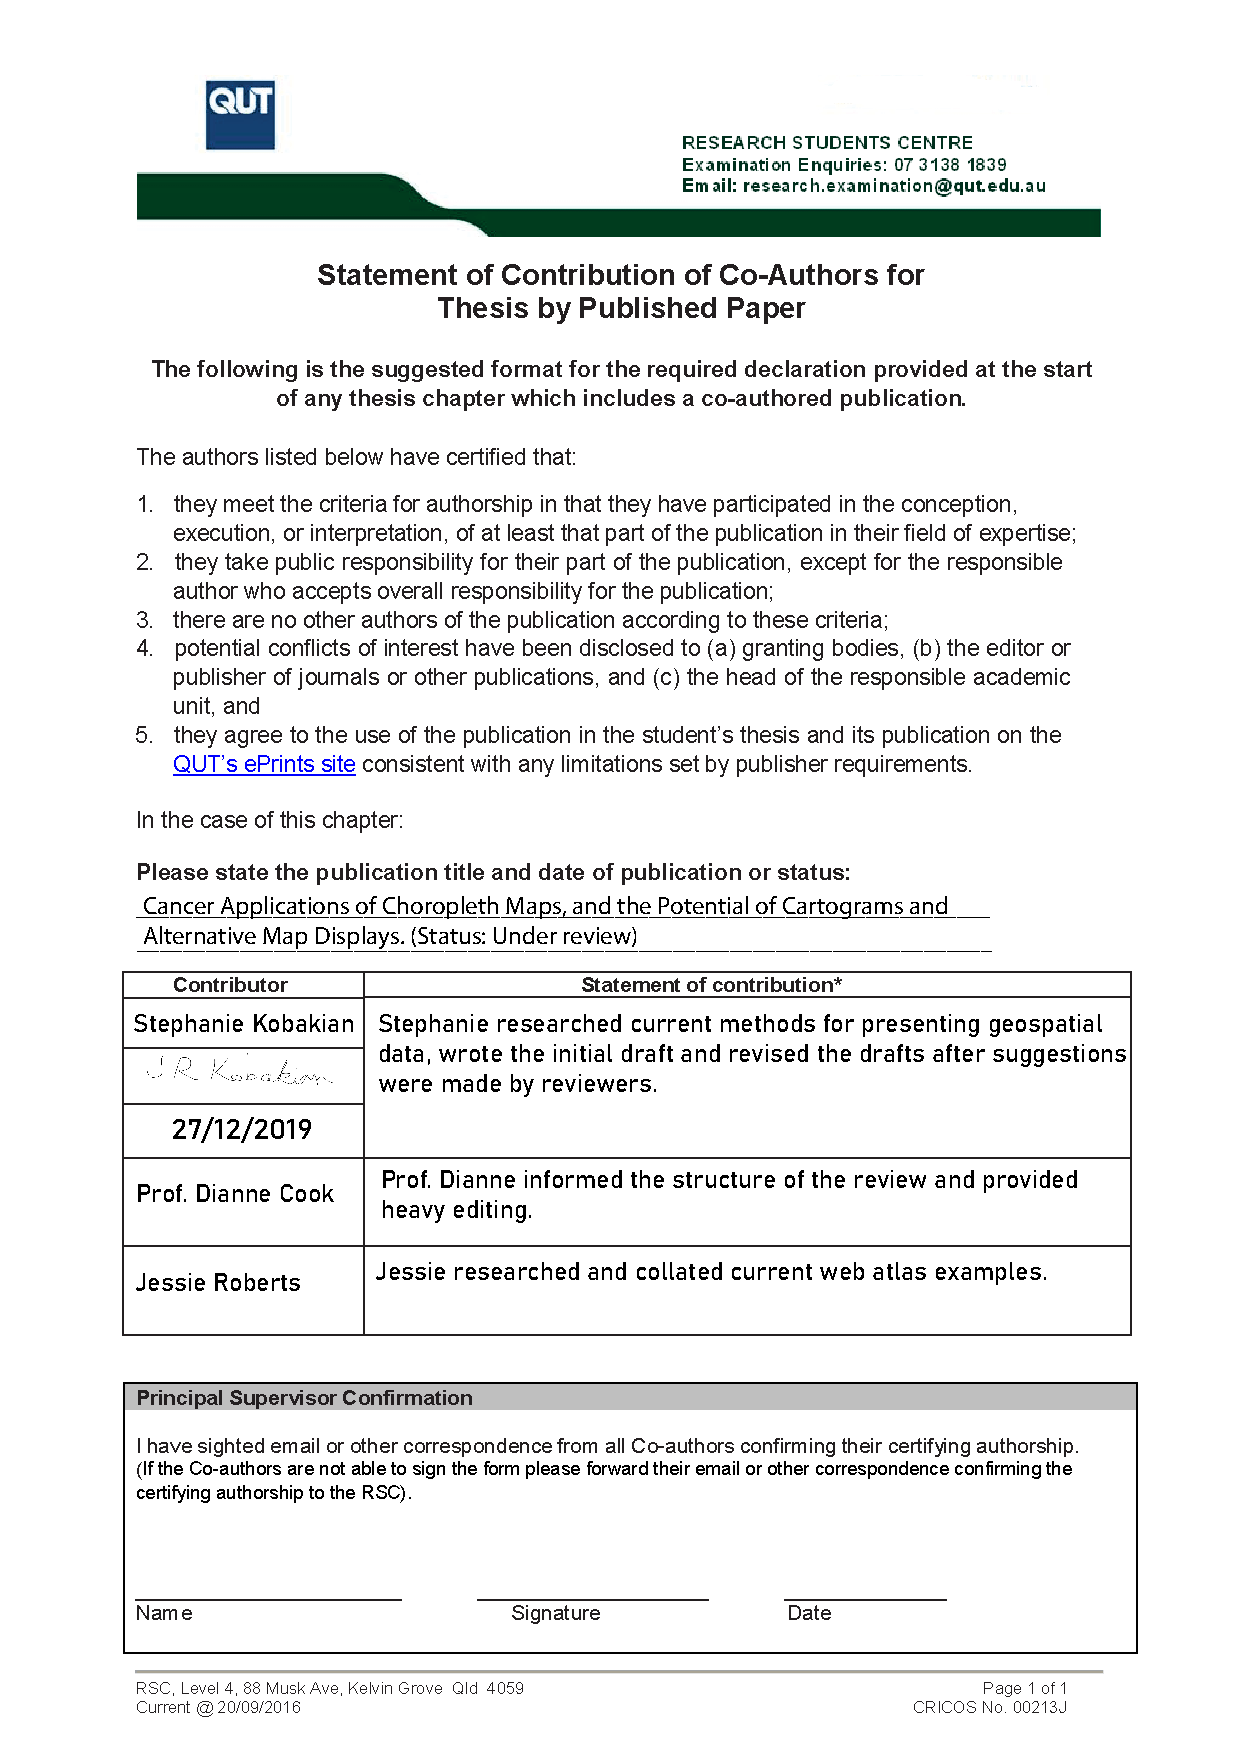
\includepdf[pages = {1-}, scale=0.8]{statement-of-contribution_literature.pdf}

\includepdf[pages = {1-}, scale=1]{02-literature.pdf}

\hypertarget{ch:algorithm}{%
\chapter{An algorithm for creating a tessellated hexagon display}\label{ch:algorithm}}

This chapter relates to the first research aim as stated in \ref{sec:aims}.
The chapter introduces the step devised for the algorithm.
The chapter frames the steps in light of the \texttt{sugarbag} \autocite{sugarbag} package functions that allow users to enact the algorithm in \texttt{R} \autocite{R}. It uses the Statisical Areas of Australia at Level 2, taking a subset and considering only those located within the island of Tasmania.
It also provides an example of how to animate between the choropleth map display and the hexagon tile map.

This chapter was submitted for publication to the \emph{Journal of Statistical Software} for publication.
The steps in this algorithm are implemented in the \texttt{sugarbag} \autocite{sugarbag} package for \texttt{R} \autocite{R}.

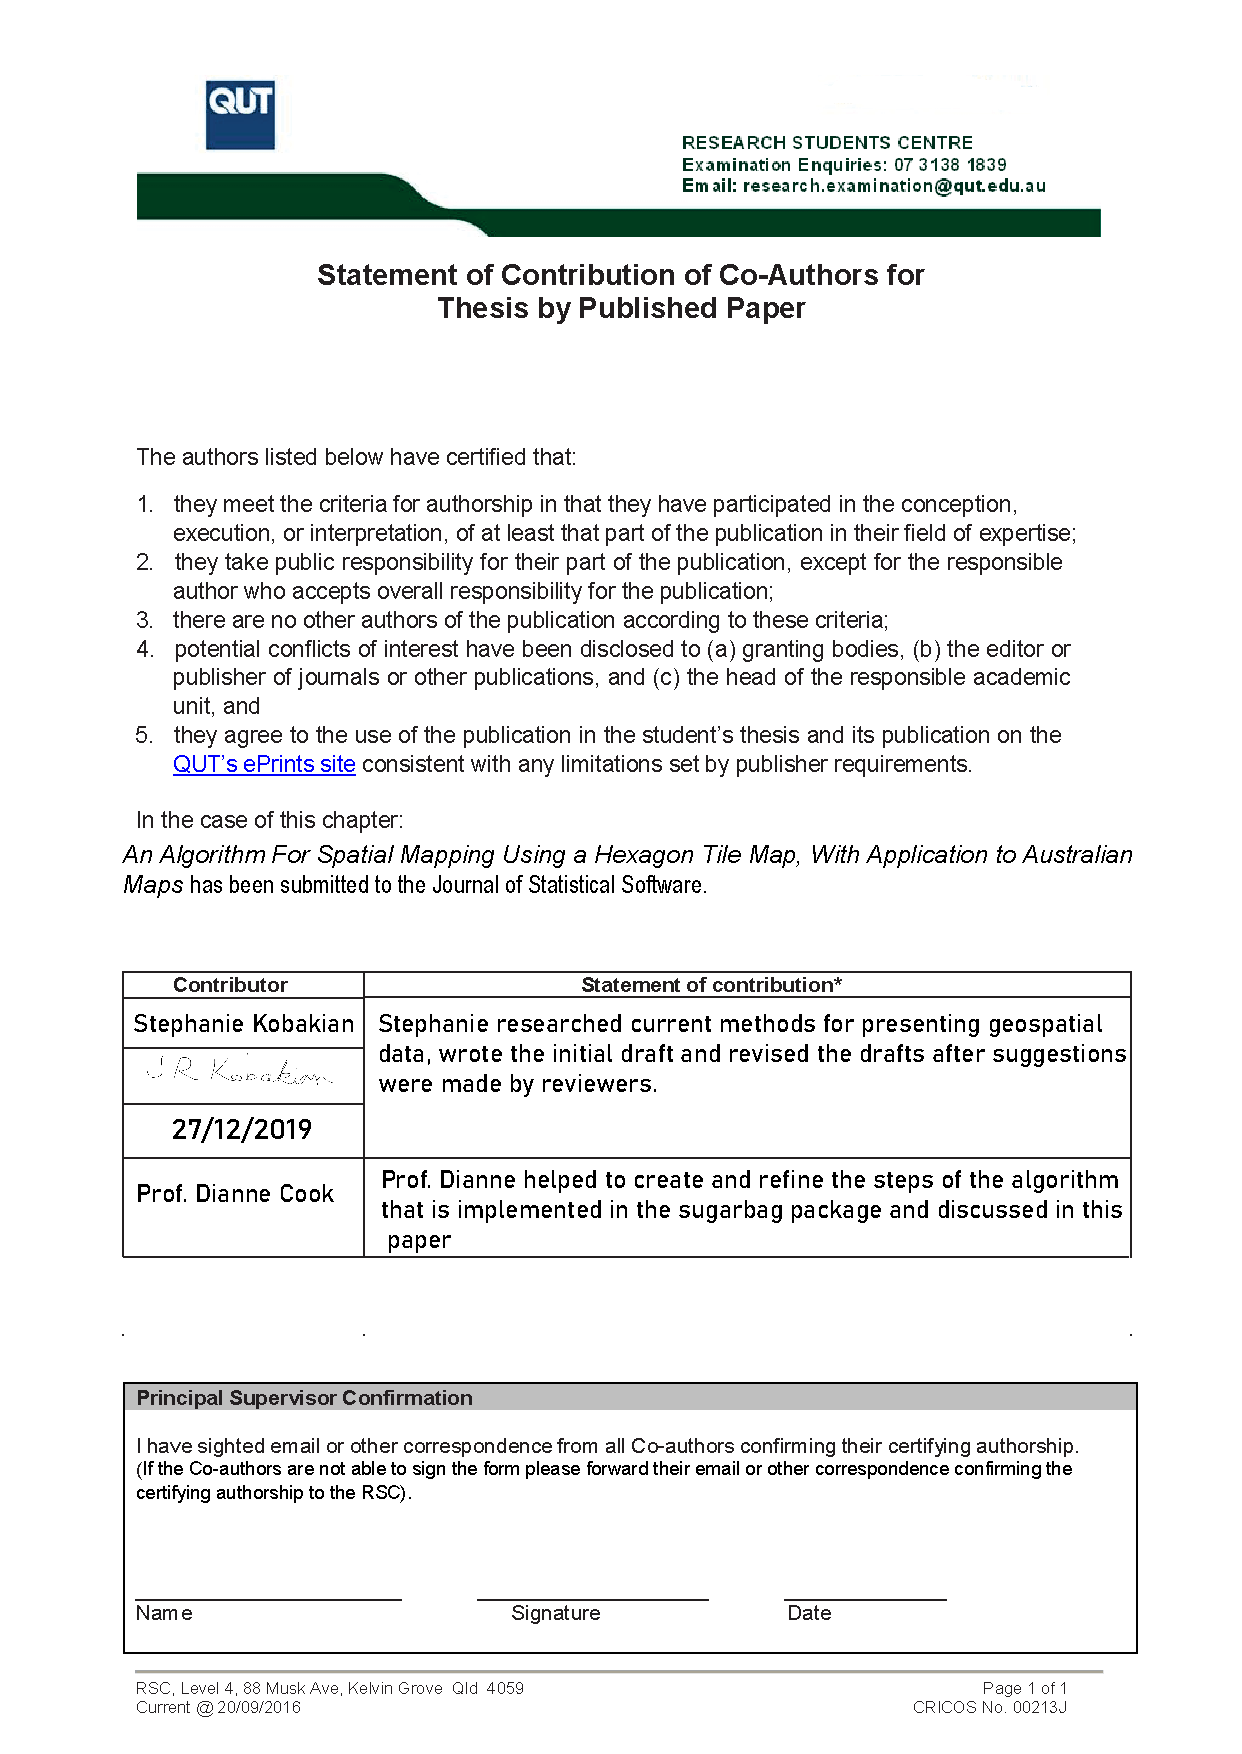
\includepdf[pages = {1-}, scale=0.8]{statement-of-contribution_algorithm.pdf}

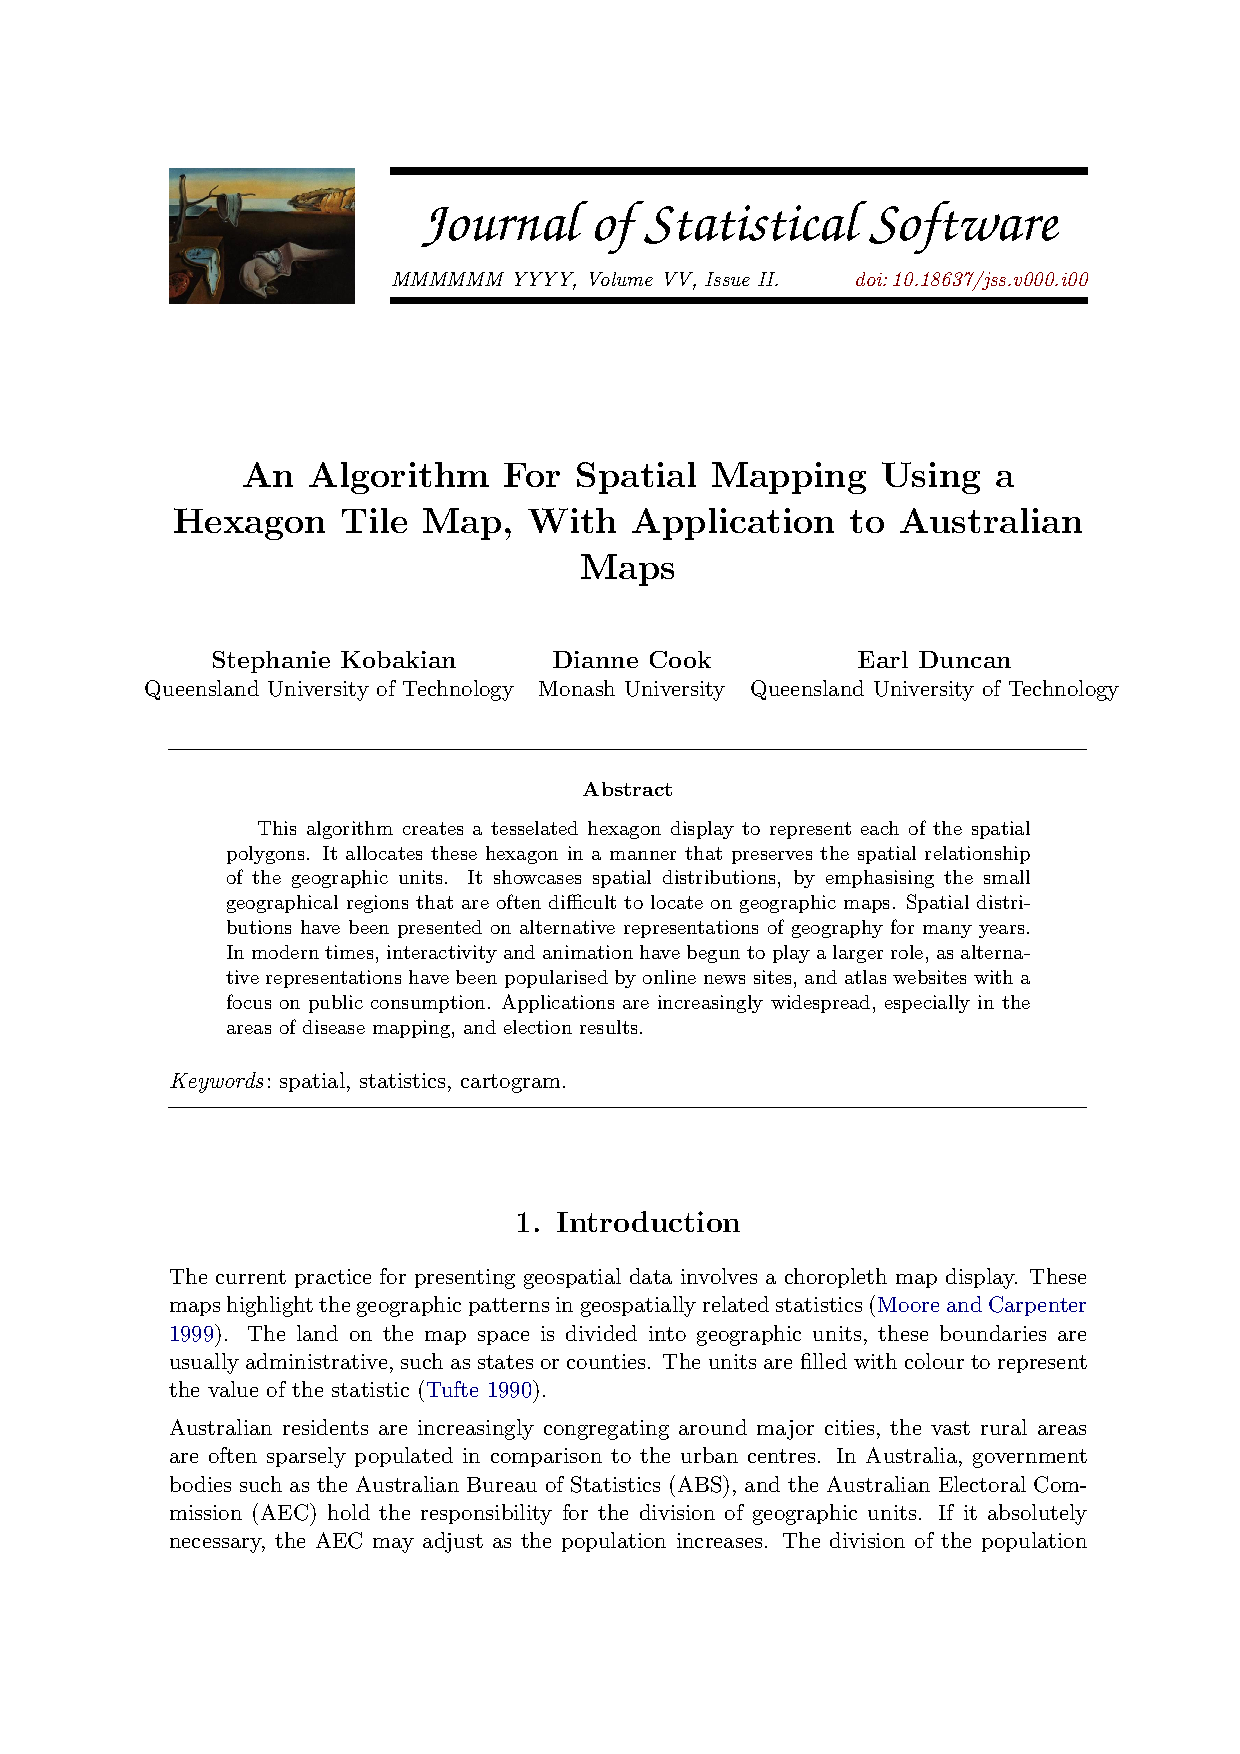
\includepdf[pages = {1-}, scale=1]{03-algorithm.pdf}

\hypertarget{ch:experiment}{%
\chapter{Visual Inference Study}\label{ch:experiment}}

This chapter tests the performance of the hexagon tile map display created using the algorithm discussed in \ref{ch:algorithm}.
It outlines the lineup protocol method of visual inference used to test information visualisations.
Using a two factor experimental design, the experiment contrasts the performance of participants when they viewed a choropleth map, and a hexagon tile map.
The contrast also involved three types of spatial trends, one geographic trend, and two population related distributions.
The results showed that participants did in fact more accurately find the population related distributions.

This chapter has been submitted to the journal \emph{IEEE Transactions of Visualisation and Computer Graphics}.

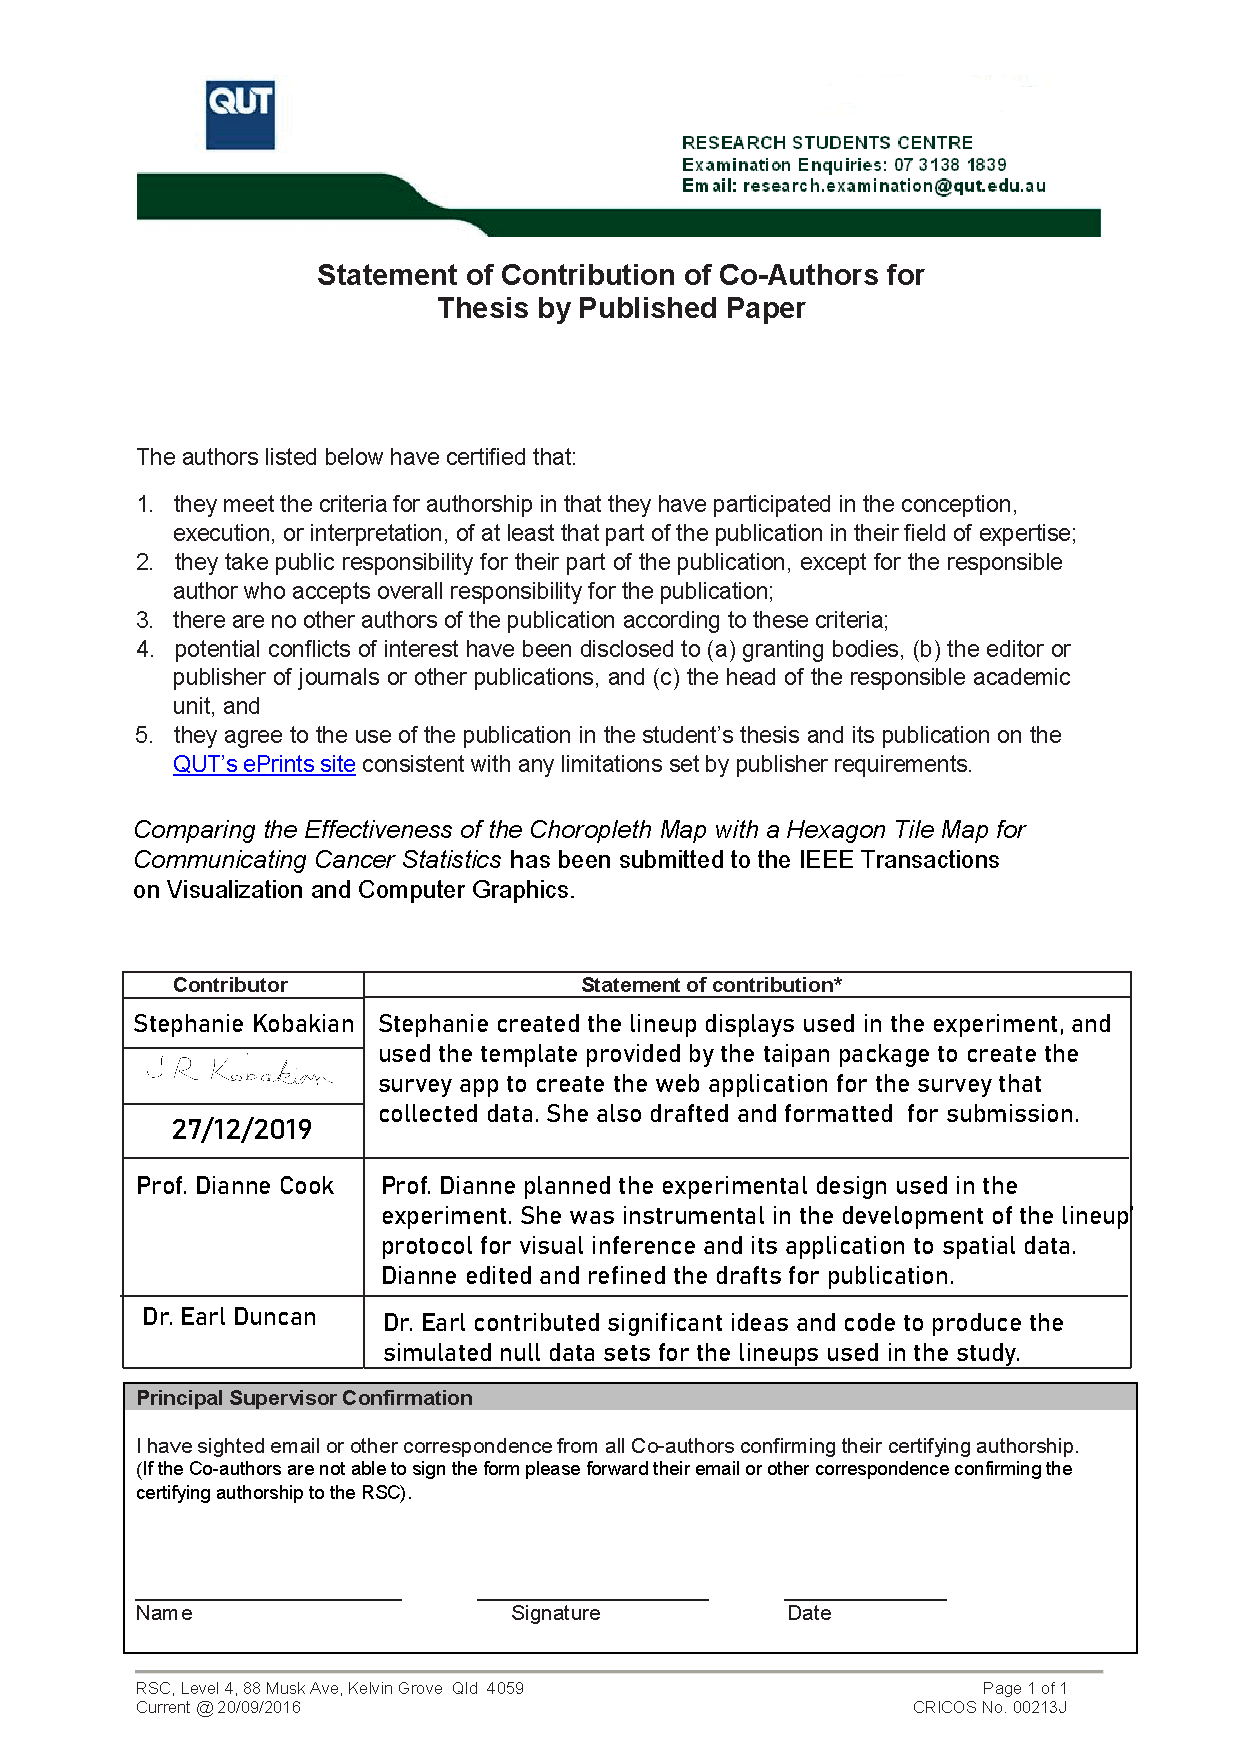
\includepdf[pages = {1-}, scale=0.8]{statement-of-contribution_experiment.pdf}

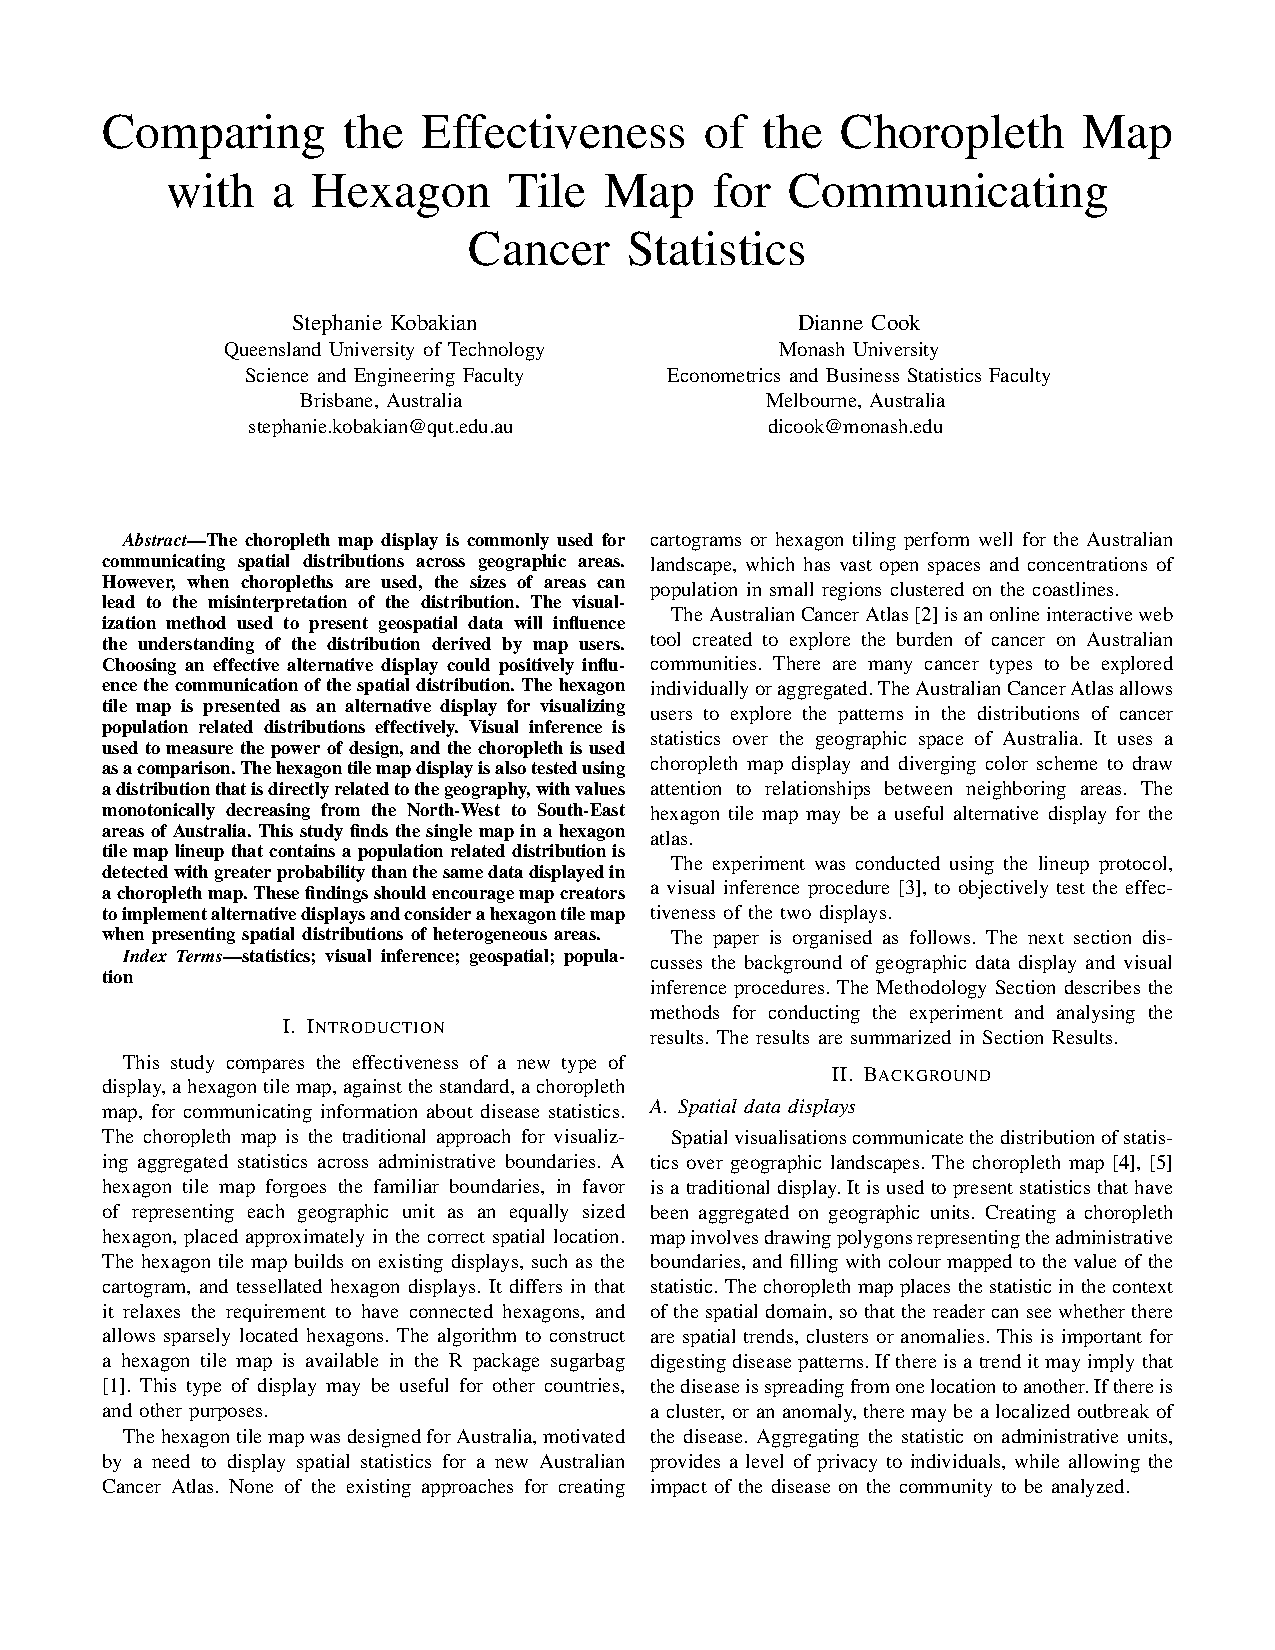
\includepdf[pages = {1-}, scale=1]{04-experiment.pdf}

\hypertarget{ch:discussion}{%
\chapter{Discussion}\label{ch:discussion}}

This chapter discusses the use of the choropleth map in presenting spatial data.
It discusses the hexagon tile map algorithm contributed by this thesis and discusses its similarities and differences from other alternative visualisation methods.
It discusses the use of the visual inference study for evaluating the displays produced by the hexagon tile map algorithm for Australia. Finally, it discusses how animating between a choropleth and hexagon display can allow map creators to direct the attention of users to the overlooked, small but densely populated geographic areas.

\hypertarget{presenting-spatial-data}{%
\section{Presenting spatial data}\label{presenting-spatial-data}}

Choropleth map displays are the traditional, and current practice method for presenting geospatial data. The use of familiar geographic polygons allows users to readily find areas of interest on the map display \autocite{EI}. The spatial patterns among the areas are revealed via the colour used to fill each geographic area.

Cancer Atlases are used to develop hypotheses about spatial distributions of cancer statistics \autocite{CPISACA}. Hot spots with high values can be detected by dramatic changes in colour between neighbours \autocite{MACM}.

However, when used as a tool communicate spatial distributions the use of the choropleth map may lead to misinterpretation of the overall distribution. This is because of the overemphasis on the large geographic areas, and the lack of visibility for the small inner-city communities \autocite{ACTUC}.

Visualisation methods have improved in iterations over many years. Cartograms \autocite{ACCAC} showed great promise and several algorithms were presented to create cartograms in the 1960s and 1970s. Cartogram techniques highlighted the population by expanding the map area of densely populated communities.
The introduction of computer assisted cartogram techniques were developed in the 1970s and 1980s. Dorling \autocite{TVSSS}, \autocite{ACTUC} introduced several alternative visualisation methods and their use has had a profound impact in the communication of data with population related distributions. These displays enabled viewers to physically see the densely populated areas and avoid spending attention on less populated, but geographically large map areas \autocite{CTTMB}.

\hypertarget{the-hexagon-tile-map-algorithm}{%
\section{The hexagon tile map algorithm}\label{the-hexagon-tile-map-algorithm}}

A key aim of this thesis was to present an algorithm for displaying geospatial data. The algorithm presented in chapter algorithm is the result of many iterations in the process necessary to transform geographic areas into a tessellated hexagon tile map.

The tessellation employed in the hexagon tile map algorithm maintains connectedness between neighbouring areas, this draws inspiration from contiguous cartograms \autocite{ACA}, rectangular cartograms \autocite{RSCW} and Dorling's circular cartograms \autocite{ACTUC}. However, the hexagon tile map algorithm does not employ the gravitation pull mathematics that is used to create contiguous cartograms. It also does not iterate on the placement of hexagons.\\
The choice of the hexagon, a consistent shape used for all areas, also draws from rectangular and Dorling cartograms. This encourages map readers to focus on the similarities or difference in the colour between geographic neighbours, and does not distract them with unfamiliar boundaries after a contiguous cartogram transformation.

The hexagon tile map display is least like the non-contiguous cartogram \autocite{NAC} which maintains the familiar geographic shapes. Some similarity in the final results may occur as densely populated regions maintain connectivity with neighbours, and sparsely populated areas will use the underlying white map space to separate neighbours.

The implementation of the \texttt{sugarbag} \autocite{sugarbag} package for R \autocite{R} provides map creators the opportunity to apply the algorithm to any set of geospatial polygons. This does not require manual creation of grids, but the displays are reusable for any populated related data set that uses the same set of geographic units.

\hypertarget{visual-inference-study-1}{%
\section{Visual inference study}\label{visual-inference-study-1}}

Conducting a visual inference study allowed a contrast of the traditional choropleth display to the alternative hexagon tile map.

The visual inference study showed that the hexagon tile map display is a valid alternative as participants achieved higher detection rates for the hexagon tile map when presenting the geographic spatial distribution and the population related distributions.

\hypertarget{animating-between-displays}{%
\section{Animating between displays}\label{animating-between-displays}}

Interactivity can allow greater detail to be drawn about small neighbourhoods in a choropleth map. By zooming in, the same shapes shown on the initial map become much larger and comparisons between immediate neighbours becomes simpler.
Interacting can also allow the map user to drive their exploration. In the case of the Australian Cancer Atlas, the interactive tools allow quick comparisons between areas far from each other on the map. It also allows quick comparisons of the estimated cancer statistics by showing the colours for each cancer type in a table-like display. These additions allow user driven exploration, but do not guarantee that the spatial distribution across the country is digested accurately.

Animating between a choropleth and a hexagon tile map will allows map users to understand how the small communities of a whole country are affected simultaneously. It also teaches map users how to find areas of interest as their attention is drawn to the capital cities, that may not have caught their attention in the display of the choropleth map. When communicating cancer statistics, there should be a balance between providing people a familiar landscape and ensuring the interpret the spatial distribution correctly. A directed exploration of a collection of inner city neighbourhoods will take the distribution out of context, the Australian Cancer Atlas provides some visual tools to combat this by highlighting that the areas displayed are only subsets However, allowing the values of an inner-city neighbourhood to be visible in the context of all other areas will enhance the understanding of the spatial distribution. Animations will communicate a specific message through the capture and direction of users' attention.

The animations created of the Australian Statistical Areas at Level 2, used in the Australian Cancer Atlas, highlight just how many SA2 areas are hidden due to their size in the choropleth display. The rapid shrinking of the rural areas allows users to recognise the emphasis that had been placed on the large geographic regions.
Their attention is then drawn to the expanding capital cities, and the coastal towns that were not previously visible.

\hypertarget{ch:conclusion}{%
\chapter{Conclusion}\label{ch:conclusion}}

The first aim of this thesis was to present an alternative visualisation method for spatial data. This thesis has provided a new algorithm to present spatial distributions of disease data, and includes an R code \autocite{R} implementation. The spatial data sets that will be effectively communicated by this display will likely have population related distributions. The hexagon tile map display will represent each area equally on the map space to effectively convey the spatial distribution of the set.

The hexagon tile map visualisation method solves the misrepresentation problem of choropleth displays of geographic data sets that contain a substantial amounts of areas. This algorithm is accessible to all R users, in a set of simple functions. It can be applied to any set of areas in an \texttt{sf} \autocite{sf} object.

The tile map allocation provided by the \texttt{allocate} function in the \texttt{sugarbag} package can easily be used to create animations between a choropleth and hexagon tile map display. Linking the familiar geography to the effective display for understanding the distribution across many heterogeneous geographic regions.

The effectiveness of the hexagon tile map has been proved by the visual inference study. It showed that participants could recognise the data display in the set of null distributions more frequently when viewing a hexagon tile map display. The choropleth map display is still effective for distributions that are directly related to the geography, such as the North-West to South-East distribution used in the study.
This has expanded the applications of visual inference studies in a spatial data context.

Future work will include expanding on criteria to evaluate the hexagon tile maps produced by the algorithm. The methods to evaluate the alternative displays have not been thoroughly explored in this thesis.
This framework will be used to create relevant tests that contrast the use of the map area, and changes in the visual statistics when the parameter of the hexagon tile map algorithm are altered.

The current hexagon tile map creates a template map that can be used to visualise any data set that contains the areas used to create the map.
There is the possibility of allowing a bivariate display to incorporate uncertainty by using a colour scheme that operates in two directions as suggested by Lucchesi and Wikle \autocite{VUADBC}.
The animation methods that allow colours filling the hexagons to flicker communicate uncertainty could also be employed.

With large hexagons, there is a potential to incorporate geofacets \autocite{IGF} to create a tessellated display of small visualisations for each geographic unit. These displays become increasingly complex if the visualisation becomes more detailed, or the hexagons become smaller.

This work has contributed a new visualisation for spatial data sets. The spatial distributions of cancer burden for different types of cancers largely relates to the population rather than the geography. The alternative visualisation method highlights the communities, and the hexagon tile map may be implemented in future iterations of the Australian Cancer Atlas to improve the communication of spatial patterns of cancer burden on Australian communities. For wide use by map creators and those interested in alternative visual displays, the code implementation has been provided to any R user with examples and documentation.
This work has also contributed to the literature of visual inference studies, by using the ``lineup'' protocol developed by Buja et al.~and used by \textcite{GIIV}, and \textcite{GTPCCD}. This example showed there was a difference in the rate of pattern recognition when participants saw competing spatial map displays.

To communicate human related spatial patterns of disease, map creators should consider the use of alternative displays. The hexagon tile map display has proven effective in this thesis for communicating spatial distributions in sets of heterogeneous geographic units. This thesis provides a practical guide for map creators communicating spatial displays of cancer data in Australia.

\appendix

\hypertarget{visual-inference-study-lineups}{%
\chapter{Visual inference study lineups}\label{visual-inference-study-lineups}}

\hypertarget{overall-performance}{%
\section{Overall Performance}\label{overall-performance}}

The detection rate is considered for each lineup. The detection rates for group A were less varied than the detection rates for the lineups seen by group B. Fig. \ref{fig:pdetection-group} shows the distribution using a boxplot. This shows the median value for detection rate was extremely similar.

\begin{figure}
\centering
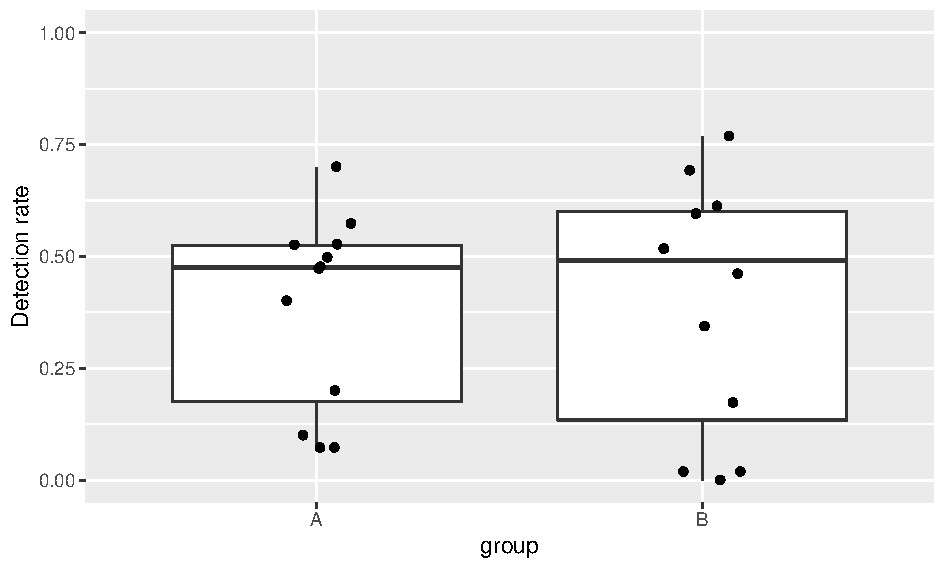
\includegraphics{thesis_files/figure-latex/pdetection-group-1.pdf}
\caption{\label{fig:pdetection-group}Boxplots of the distribution of detection rates for each line up, separated by group.}
\end{figure}

The overall detection rate is considered for each trend model in Fig. \ref{fig:pdetect-trend}.
The detection rates for the NW-SE trend model was less varied than the detection rates for the Three Cities and All Cities trends. Fig. \ref{fig:pdetection-group} shows the distribution using a boxplot. This shows the distributions of the rates do not overlap for NW-SE and Three Cities trends, the Three cities range was larger, but the median was much higher for the NW-SE trend. The All Cities trend model distribution overlaps with the NW-SE and All Cities trends.

\begin{figure}
\centering
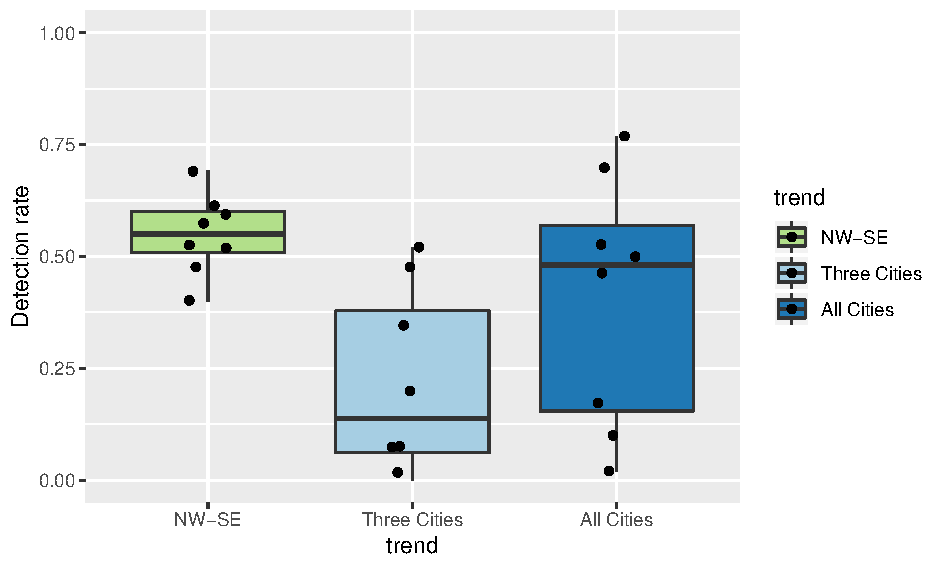
\includegraphics{thesis_files/figure-latex/pdetect-trend-1.pdf}
\caption{\label{fig:pdetect-trend}Boxplots of the distribution of detection rates for each line up, separated by trend model.}
\end{figure}

The boxplots in Fig. \ref{fig:pdetection-type} contrast the distribution of the detection rates for eah type of display.
The detection rates across the lineups was less varied for the hexagon display. There was a large difference in the medians for the types of displays.
Without considering the relationship for each lineup, the hexagon lineup display allowed the participants to achieve higher detection rates.

\begin{figure}
\centering
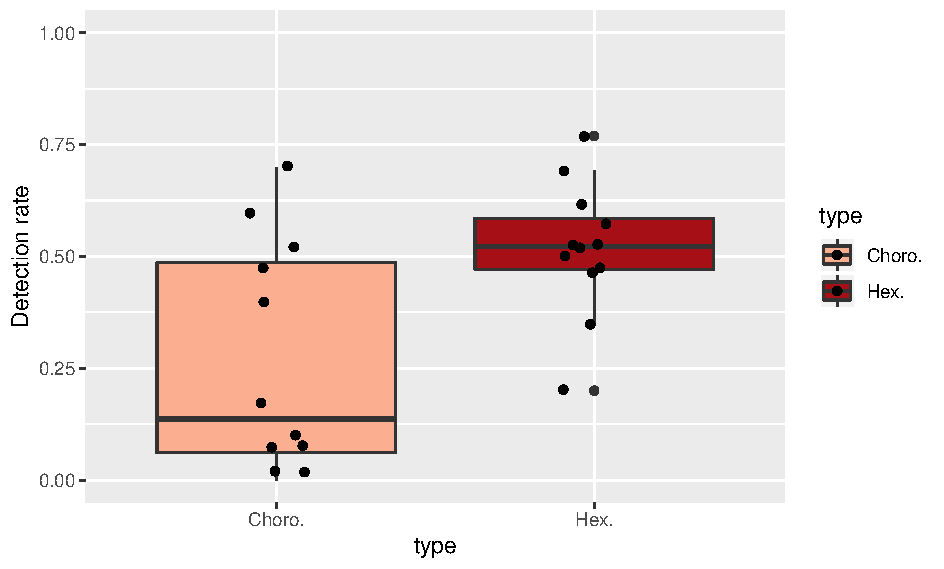
\includegraphics{thesis_files/figure-latex/pdetection-type-1.pdf}
\caption{\label{fig:pdetection-type}Boxplots of the distribution of detection rates for each line up, separated by type of display.}
\end{figure}

\hypertarget{lineups}{%
\section{Lineups}\label{lineups}}

Each lineup had twelve map displays, this gave participants the choice of any plot, and the choice to not provide a response. this non-reponse is indicated by 0.
The choices made by participants are displayed in Fig. \ref{fig:choices}. The height of each orange lollipop indiates the proportion of participants that selected the map display of real data, they represent the correct choices.
The green lollipops show the proportion of participants that selected the incorrect displays in each lineup.

The proportion of choices are also presented separately for each trend model in Table. \ref{tab:choice-nwse}, Table. \ref{tab:choice-three}, and Table. \ref{tab:choice-all}.
The correct map display in lineups with a North West to South East trend was chosen correctly with much greater frequency.
In the lineups of All Cities displays, participants were misled by the choropleth display, but not the hexagon display for all except (2).
All of Three Cities displays, except (4), were detected in the hexagon display. All except one lineup had at least one participant select the correct map in the lineup as shown in Fig. \ref{fig:choices}.

\begin{figure}
\centering
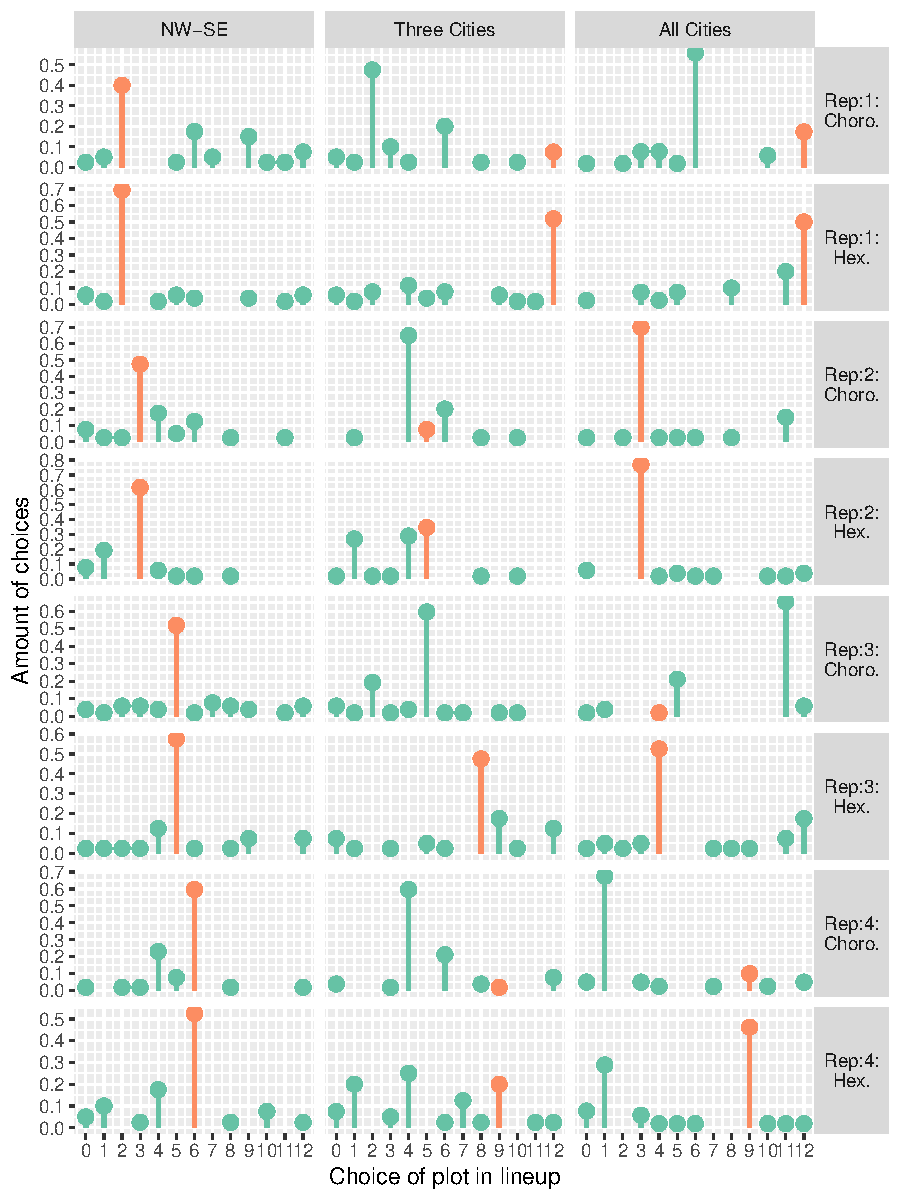
\includegraphics{thesis_files/figure-latex/choices-1.pdf}
\caption{\label{fig:choices}Pin plots of the propotion of choices made for each lineup location. Each facet is associated with one lineup, the height of the points show the proportion of the participants that made each choice when considering each lineup. The points coloured orange show the map which contained a trend model, these are the correct choices. The numbers differentiate the replicates of each trend model and type of map display. Participants were able to select 0 to indicate they did not want to choose a map.}
\end{figure}

\begin{table}

\caption{\label{tab:choice-nwse}The proportion of participants who selected each of the twelve map choices in each lineup for NW-SE displays.}
\centering
\begin{tabular}[t]{r|r|r|r|r|r|r|r|r|r|r|r|r|r|r}
\hline
Rep & Type & 0 & 1 & 2 & 3 & 4 & 5 & 6 & 7 & 8 & 9 & 10 & 11 & 12\\
\hline
 & Choro. & 0.02 & 0.05 & 0.4 & 0 & 0 & 0.02 & 0.18 & 0.05 & 0 & 0.15 & 0.02 & 0.02 & 0.08\\
\cline{2-15}
\multirow{-2}{*}{\raggedleft\arraybackslash 1} & Hex. & 0.06 & 0.02 & 0.69 & 0 & 0.02 & 0.06 & 0.04 & 0 & 0 & 0.04 & 0 & 0.02 & 0.06\\
\cline{1-15}
 & Choro. & 0.08 & 0.02 & 0.02 & 0.48 & 0.18 & 0.05 & 0.12 & 0 & 0.02 & 0 & 0 & 0.02 & 0\\
\cline{2-15}
\multirow{-2}{*}{\raggedleft\arraybackslash 2} & Hex. & 0.08 & 0.19 & 0 & 0.62 & 0.06 & 0.02 & 0.02 & 0 & 0.02 & 0 & 0 & 0 & 0\\
\cline{1-15}
 & Choro. & 0.04 & 0.02 & 0.06 & 0.06 & 0.04 & 0.52 & 0.02 & 0.08 & 0.06 & 0.04 & 0 & 0.02 & 0.06\\
\cline{2-15}
\multirow{-2}{*}{\raggedleft\arraybackslash 3} & Hex. & 0.02 & 0.02 & 0.02 & 0.02 & 0.12 & 0.57 & 0.02 & 0 & 0.02 & 0.08 & 0 & 0 & 0.08\\
\cline{1-15}
 & Choro. & 0.02 & 0 & 0.02 & 0.02 & 0.23 & 0.08 & 0.6 & 0 & 0.02 & 0 & 0 & 0 & 0.02\\
\cline{2-15}
\multirow{-2}{*}{\raggedleft\arraybackslash 4} & Hex. & 0.05 & 0.1 & 0 & 0.02 & 0.18 & 0 & 0.52 & 0 & 0.02 & 0 & 0.08 & 0 & 0.02\\
\hline
\end{tabular}
\end{table}

\begin{table}

\caption{\label{tab:choice-three}The proportion of participants who selected each of the twelve map choices in each lineup for Three Cities displays.}
\centering
\begin{tabular}[t]{r|r|r|r|r|r|r|r|r|r|r|r|r|r|r}
\hline
Rep & Type & 0 & 1 & 2 & 3 & 4 & 5 & 6 & 7 & 8 & 9 & 10 & 11 & 12\\
\hline
 & Choro. & 0.05 & 0.02 & 0.48 & 0.1 & 0.02 & 0 & 0.2 & 0 & 0.02 & 0 & 0.02 & 0 & 0.08\\
\cline{2-15}
\multirow{-2}{*}{\raggedleft\arraybackslash 1} & Hex. & 0.06 & 0.02 & 0.08 & 0 & 0.12 & 0.04 & 0.08 & 0 & 0 & 0.06 & 0.02 & 0.02 & 0.52\\
\cline{1-15}
 & Choro. & 0 & 0.02 & 0 & 0 & 0.65 & 0.08 & 0.2 & 0 & 0.02 & 0 & 0.02 & 0 & 0\\
\cline{2-15}
\multirow{-2}{*}{\raggedleft\arraybackslash 2} & Hex. & 0.02 & 0.27 & 0.02 & 0.02 & 0.29 & 0.35 & 0 & 0 & 0.02 & 0 & 0.02 & 0 & 0\\
\cline{1-15}
 & Choro. & 0.06 & 0.02 & 0.19 & 0.02 & 0.04 & 0.6 & 0.02 & 0.02 & 0 & 0.02 & 0.02 & 0 & 0\\
\cline{2-15}
\multirow{-2}{*}{\raggedleft\arraybackslash 3} & Hex. & 0.08 & 0.02 & 0 & 0.02 & 0 & 0.05 & 0.02 & 0 & 0.48 & 0.18 & 0.02 & 0 & 0.12\\
\cline{1-15}
 & Choro. & 0.04 & 0 & 0 & 0.02 & 0.6 & 0 & 0.21 & 0 & 0.04 & 0.02 & 0 & 0 & 0.08\\
\cline{2-15}
\multirow{-2}{*}{\raggedleft\arraybackslash 4} & Hex. & 0.08 & 0.2 & 0 & 0.05 & 0.25 & 0 & 0.02 & 0.12 & 0.02 & 0.2 & 0 & 0.02 & 0.02\\
\hline
\end{tabular}
\end{table}

\begin{table}

\caption{\label{tab:choice-all}The proportion of participants who selected each of the twelve map choices in each lineup for All Cities displays.}
\centering
\begin{tabular}[t]{r|r|r|r|r|r|r|r|r|r|r|r|r|r|r}
\hline
Rep & Type & 0 & 1 & 2 & 3 & 4 & 5 & 6 & 7 & 8 & 9 & 10 & 11 & 12\\
\hline
 & Choro. & 0.02 & 0 & 0.02 & 0.08 & 0.08 & 0.02 & 0.56 & 0 & 0 & 0 & 0.06 & 0 & 0.17\\
\cline{2-15}
\multirow{-2}{*}{\raggedleft\arraybackslash 1} & Hex. & 0.02 & 0 & 0 & 0.08 & 0.02 & 0.08 & 0 & 0 & 0.1 & 0 & 0 & 0.2 & 0.5\\
\cline{1-15}
 & Choro. & 0.02 & 0 & 0.02 & 0.7 & 0.02 & 0.02 & 0.02 & 0 & 0.02 & 0 & 0 & 0.15 & 0\\
\cline{2-15}
\multirow{-2}{*}{\raggedleft\arraybackslash 2} & Hex. & 0.06 & 0 & 0 & 0.77 & 0.02 & 0.04 & 0.02 & 0.02 & 0 & 0 & 0.02 & 0.02 & 0.04\\
\cline{1-15}
 & Choro. & 0.02 & 0.04 & 0 & 0 & 0.02 & 0.21 & 0 & 0 & 0 & 0 & 0 & 0.65 & 0.06\\
\cline{2-15}
\multirow{-2}{*}{\raggedleft\arraybackslash 3} & Hex. & 0.02 & 0.05 & 0.02 & 0.05 & 0.52 & 0 & 0 & 0.02 & 0.02 & 0.02 & 0 & 0.08 & 0.18\\
\cline{1-15}
 & Choro. & 0.05 & 0.68 & 0 & 0.05 & 0.02 & 0 & 0 & 0.02 & 0 & 0.1 & 0.02 & 0 & 0.05\\
\cline{2-15}
\multirow{-2}{*}{\raggedleft\arraybackslash 4} & Hex. & 0.08 & 0.29 & 0 & 0.06 & 0.02 & 0.02 & 0.02 & 0 & 0 & 0.46 & 0.02 & 0.02 & 0.02\\
\hline
\end{tabular}
\end{table}

\hypertarget{north-west---south-east}{%
\section{North West - South East}\label{north-west---south-east}}

The same data set is visualised in both displays, the difference is the land area of each SA3 is coloured in the choropleth and the hexagon representing the SA3 is coloured in the Hexagon Tile Map.

Lineups were created using the Australian Statistical Areas at Level 3.

\hypertarget{all-cities}{%
\section{All Cities}\label{all-cities}}

\hypertarget{replicate-1}{%
\subsection{Replicate 1}\label{replicate-1}}

\begin{figure}
\centering
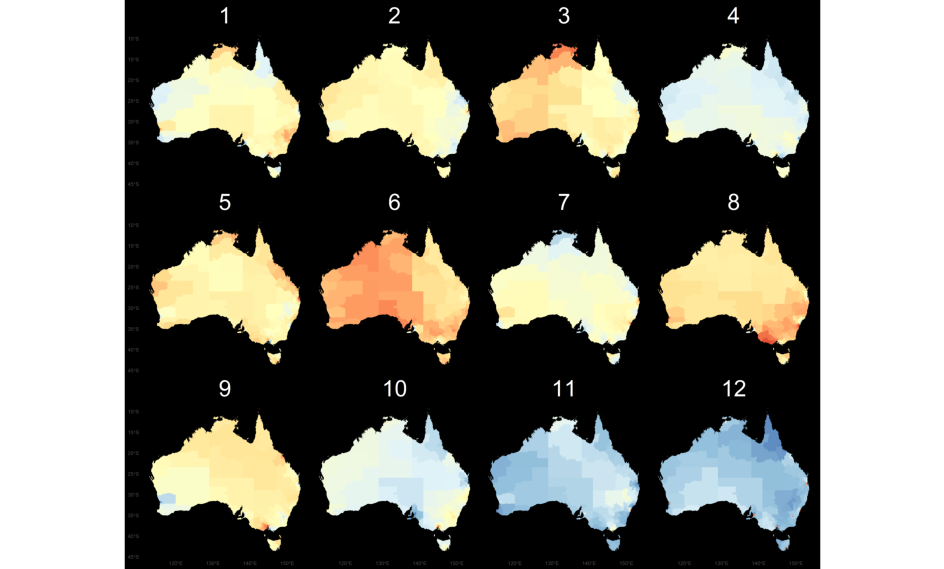
\includegraphics{thesis_files/figure-latex/cities-geo12-1.pdf}
\caption{\label{fig:cities-geo12}The lineup of choropleth map displays, location 12 contains a distribution that affects all capital cities.}
\end{figure}

\begin{figure}
\centering
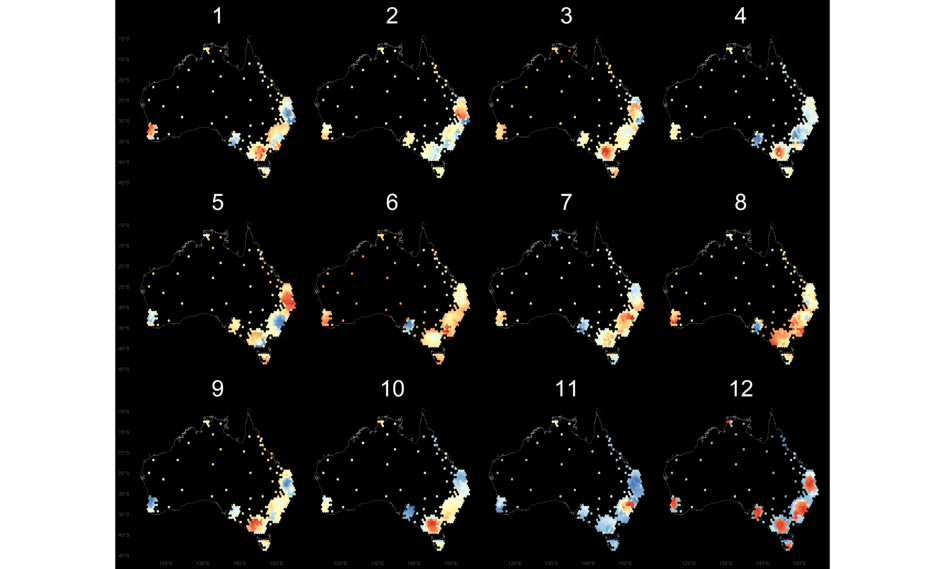
\includegraphics{thesis_files/figure-latex/cities-hex12-1.pdf}
\caption{\label{fig:cities-hex12}The lineup of hexagon tile map displays, location 12 contains a distribution that affects all capital cities.}
\end{figure}

\hypertarget{replicate-2}{%
\subsection{Replicate 2}\label{replicate-2}}

\begin{figure}
\centering
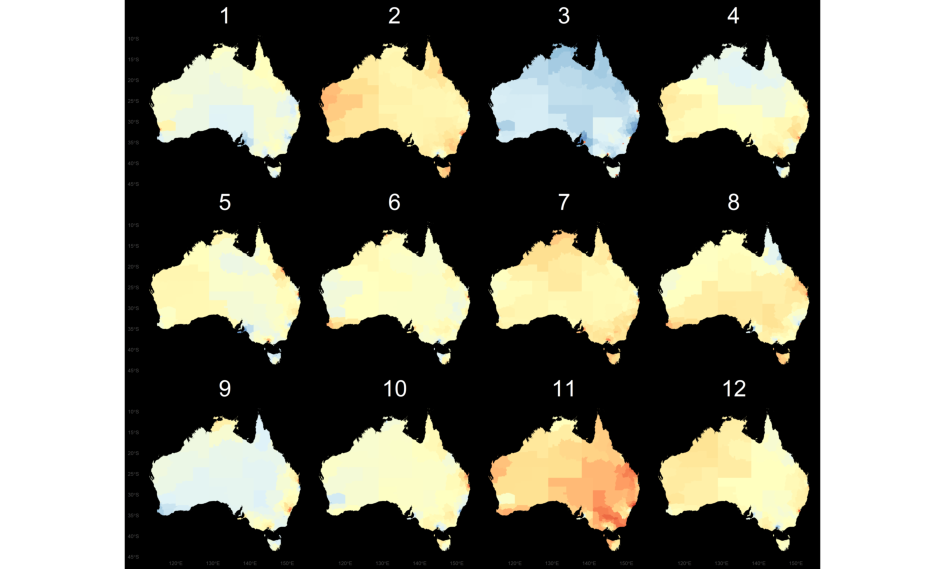
\includegraphics{thesis_files/figure-latex/cities-geo3-1.pdf}
\caption{\label{fig:cities-geo3}The lineup of choropleth map displays, location 3 contains a distribution that affects all capital cities.}
\end{figure}

\begin{figure}
\centering
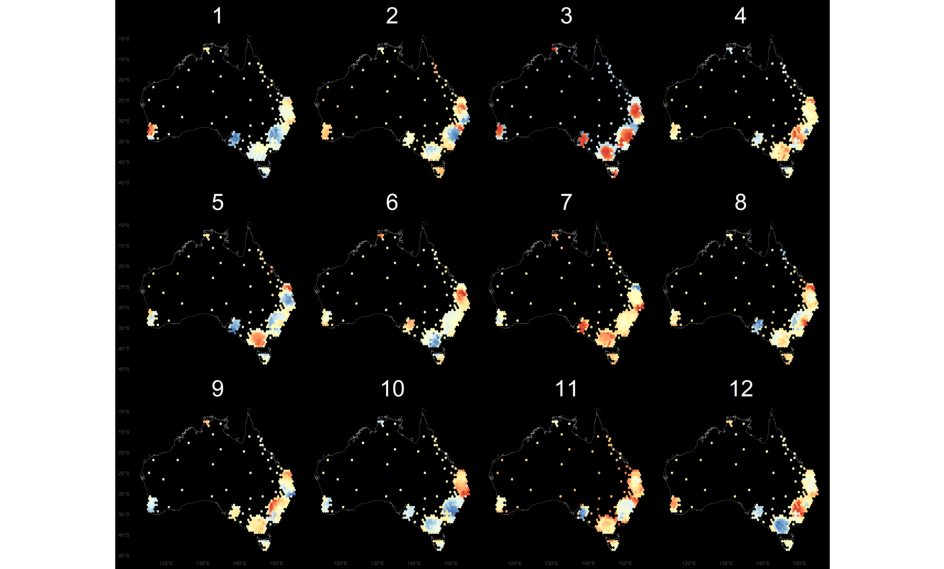
\includegraphics{thesis_files/figure-latex/cities-hex3-1.pdf}
\caption{\label{fig:cities-hex3}The lineup of hexagon tile map displays, location 3 contains a distribution that affects all capital cities.}
\end{figure}

\hypertarget{replicate-3}{%
\subsection{Replicate 3}\label{replicate-3}}

\begin{figure}
\centering
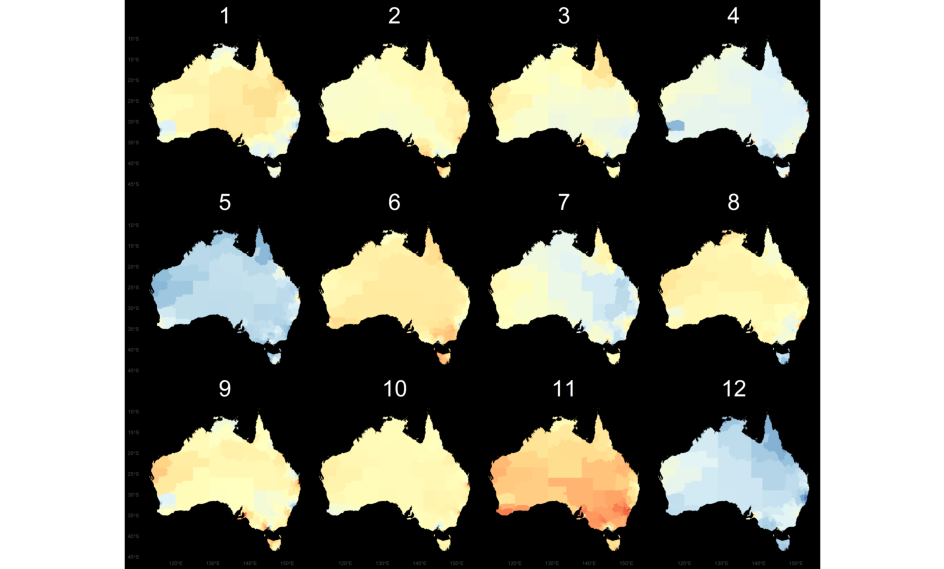
\includegraphics{thesis_files/figure-latex/cities-geo4-1.pdf}
\caption{\label{fig:cities-geo4}The lineup of choropleth map displays, location 4 contains a distribution that affects all capital cities.}
\end{figure}

\begin{figure}
\centering
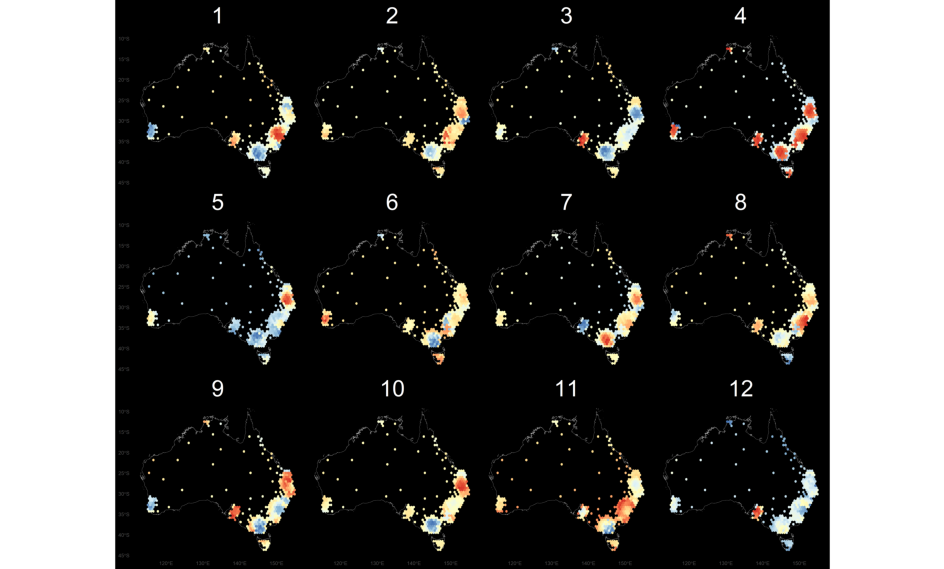
\includegraphics{thesis_files/figure-latex/cities-hex4-1.pdf}
\caption{\label{fig:cities-hex4}The lineup of hexagon tile map displays, location 4 contains a distribution that affects all capital cities.}
\end{figure}

\hypertarget{replicate-4}{%
\subsection{Replicate 4}\label{replicate-4}}

\begin{figure}
\centering
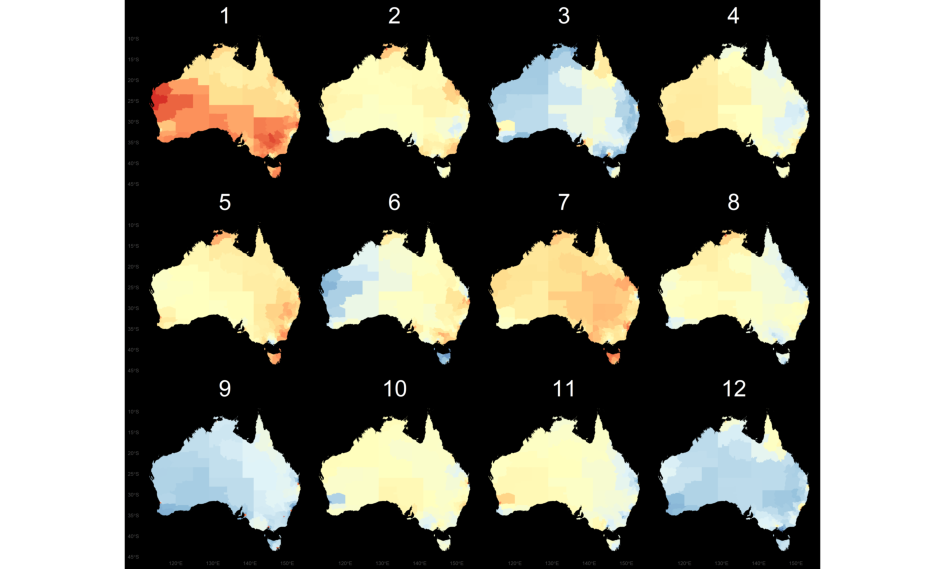
\includegraphics{thesis_files/figure-latex/cities-geo9-1.pdf}
\caption{\label{fig:cities-geo9}The lineup of choropleth map displays, location 9 contains a distribution that affects all capital cities.}
\end{figure}

\begin{figure}
\centering
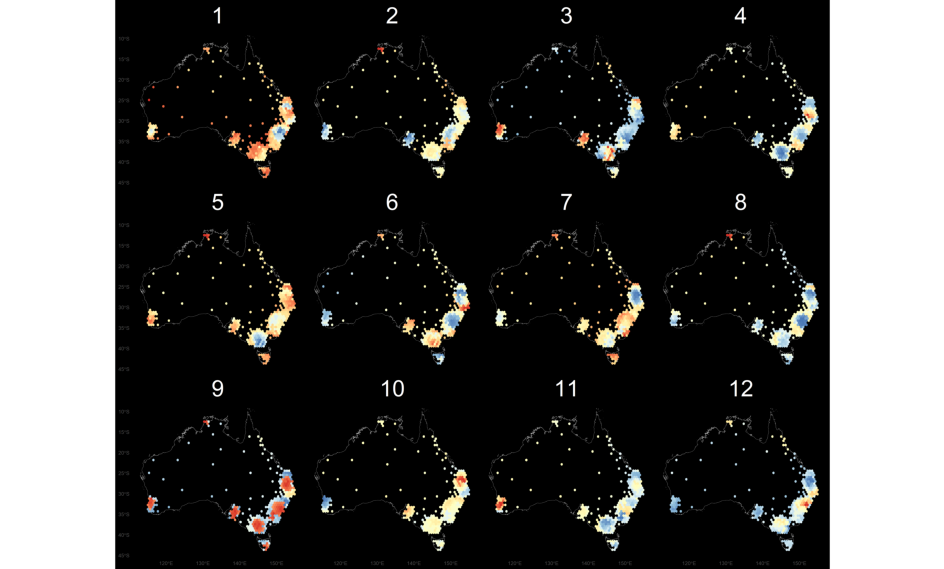
\includegraphics{thesis_files/figure-latex/cities-hex9-1.pdf}
\caption{\label{fig:cities-hex9}The lineup of hexagon tile map displays, location 9 contains a distribution that affects all capital cities.}
\end{figure}

\hypertarget{three-cities}{%
\section{Three Cities}\label{three-cities}}

\hypertarget{replicate-1-1}{%
\subsection{Replicate 1}\label{replicate-1-1}}

\begin{figure}
\centering
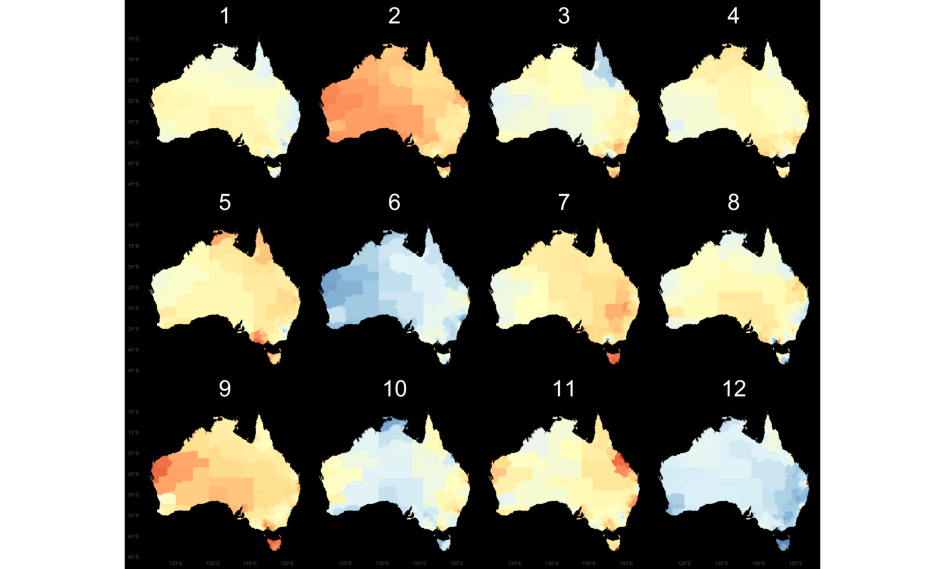
\includegraphics{thesis_files/figure-latex/three-geo12-1.pdf}
\caption{\label{fig:three-geo12}The lineup of choropleth map displays, location 12 contains a distribution that affects three of the Australian capital cities.}
\end{figure}

\begin{figure}
\centering
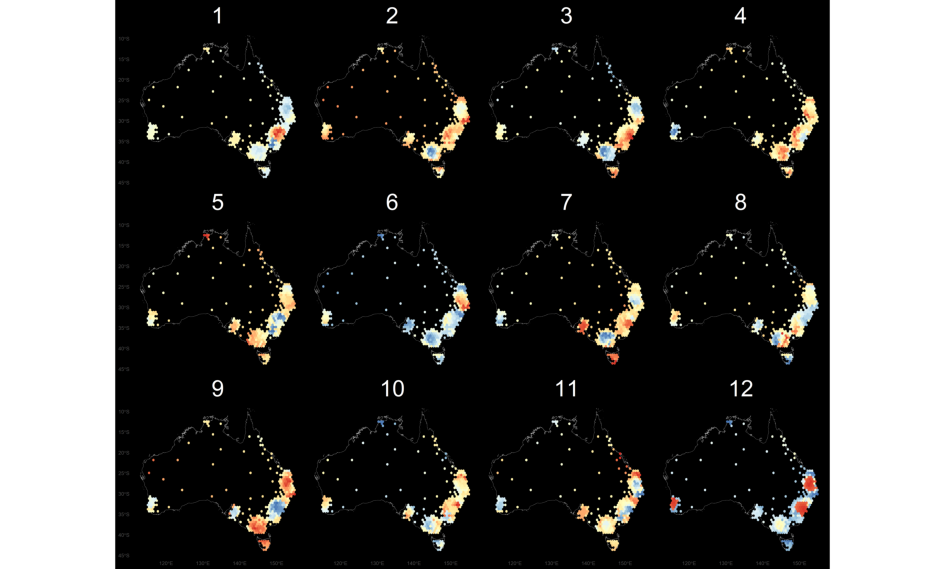
\includegraphics{thesis_files/figure-latex/three-hex12-1.pdf}
\caption{\label{fig:three-hex12}The lineup of hexagon tile map displays, location 12 contains a distribution that affects three of the Australian capital cities.}
\end{figure}

\hypertarget{replicate-2-1}{%
\subsection{Replicate 2}\label{replicate-2-1}}

\begin{figure}
\centering
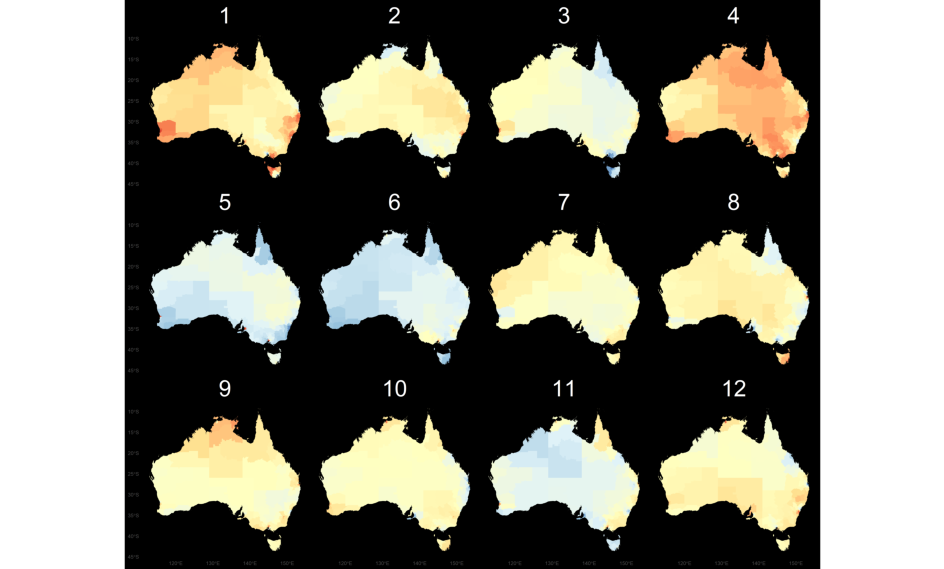
\includegraphics{thesis_files/figure-latex/three-geo5-1.pdf}
\caption{\label{fig:three-geo5}The lineup of choropleth map displays, location 3 contains a distribution that affects three of the Australian capital cities.}
\end{figure}

\begin{figure}
\centering
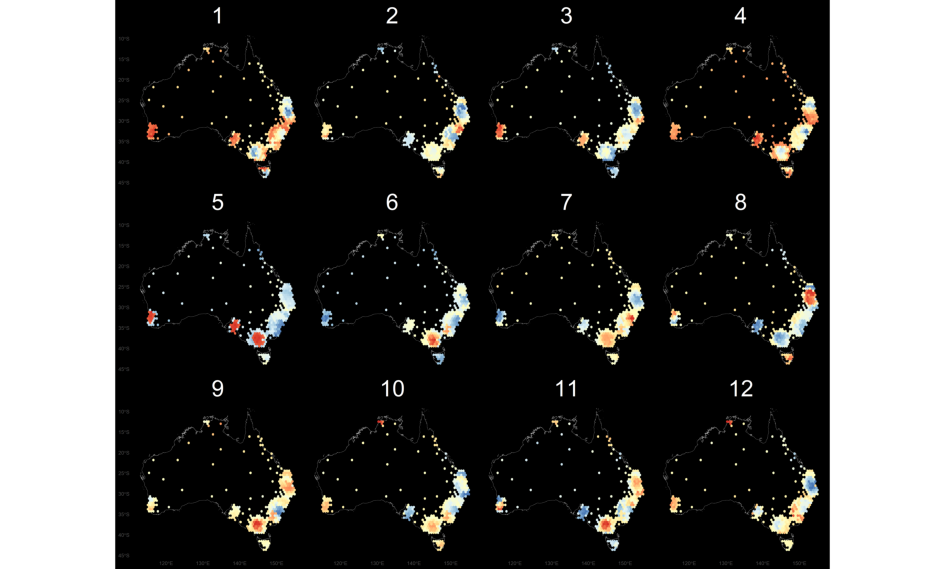
\includegraphics{thesis_files/figure-latex/three-hex5-1.pdf}
\caption{\label{fig:three-hex5}The lineup of hexagon tile map displays, location 3 contains a distribution that affects three of the Australian capital cities.}
\end{figure}

\hypertarget{replicate-3-1}{%
\subsection{Replicate 3}\label{replicate-3-1}}

\begin{figure}
\centering
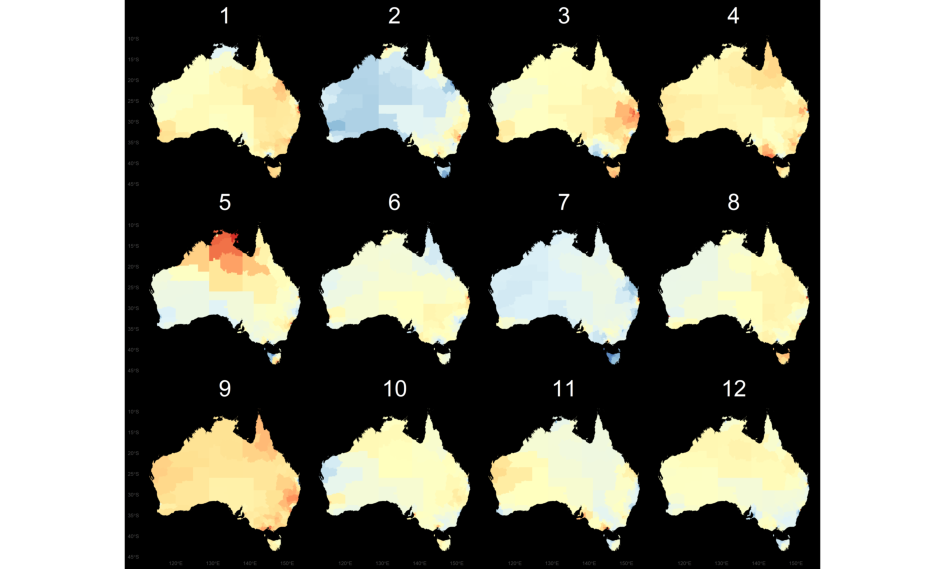
\includegraphics{thesis_files/figure-latex/three-geo8-1.pdf}
\caption{\label{fig:three-geo8}The lineup of choropleth map displays, location 4 contains a distribution that affects three of the Australian capital cities.}
\end{figure}

\begin{figure}
\centering
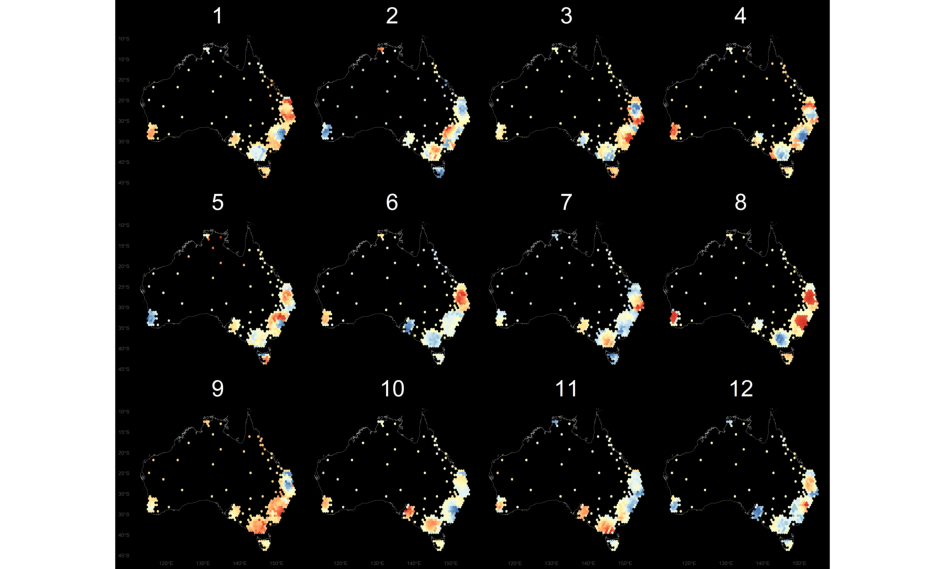
\includegraphics{thesis_files/figure-latex/three-hex8-1.pdf}
\caption{\label{fig:three-hex8}The lineup of hexagon tile map displays, location 4 contains a distribution that affects three of the Australian capital cities.}
\end{figure}

\hypertarget{replicate-4-1}{%
\subsection{Replicate 4}\label{replicate-4-1}}

\begin{figure}
\centering
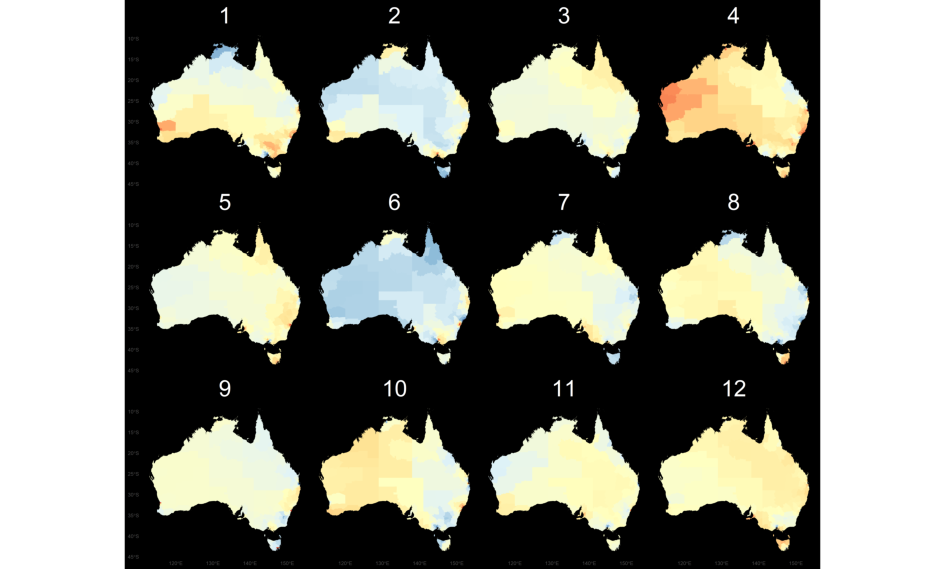
\includegraphics{thesis_files/figure-latex/three-geo9-1.pdf}
\caption{\label{fig:three-geo9}The lineup of choropleth map displays, location 9 contains a distribution that affects three of the Australian capital cities.}
\end{figure}

\begin{figure}
\centering
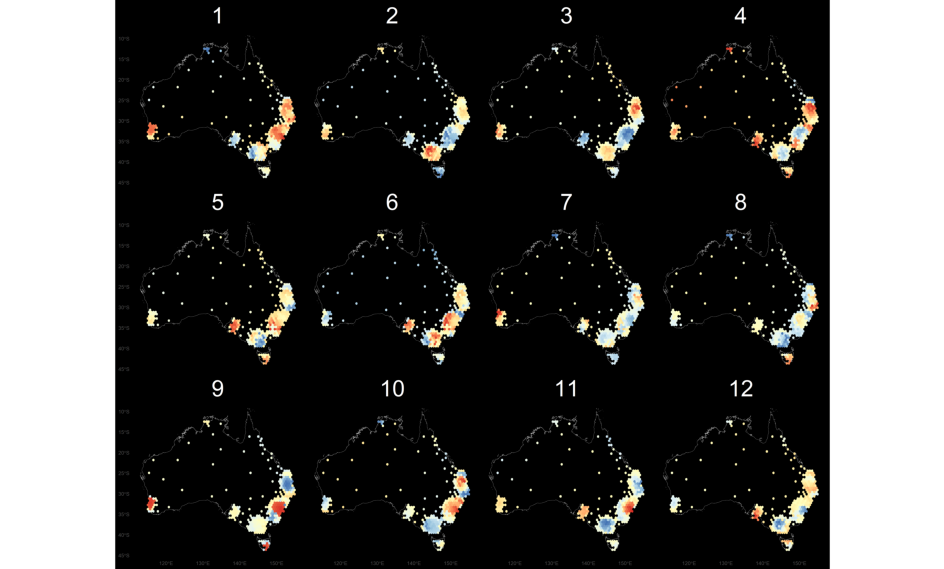
\includegraphics{thesis_files/figure-latex/three-hex9-1.pdf}
\caption{\label{fig:three-hex9}The lineup of hexagon tile map displays, location 9 contains a distribution that affects three of the Australian capital cities.}
\end{figure}

\hypertarget{north-west-to-south-east-geographic-trend}{%
\section{North West to South East Geographic Trend}\label{north-west-to-south-east-geographic-trend}}

\hypertarget{replicate-1-2}{%
\subsection{Replicate 1}\label{replicate-1-2}}

\begin{figure}
\centering
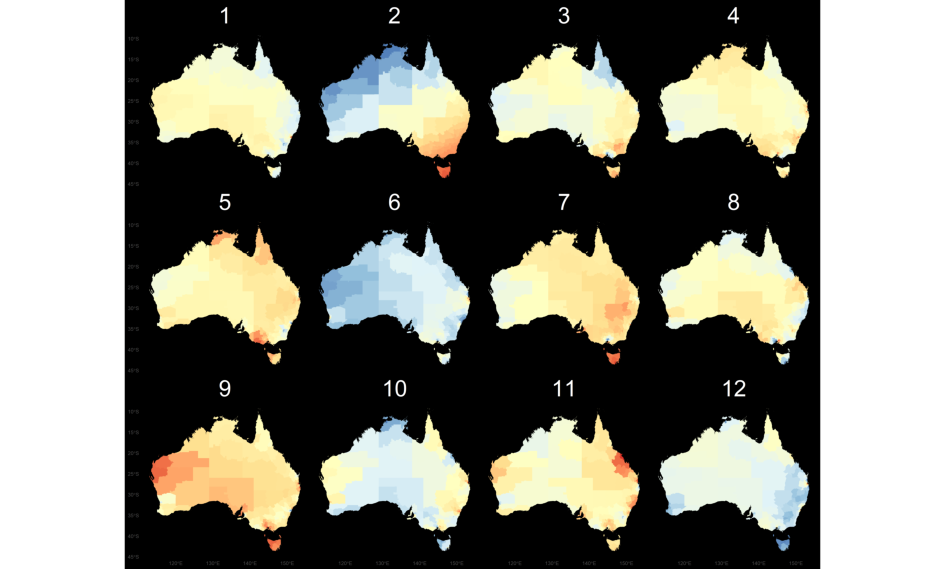
\includegraphics{thesis_files/figure-latex/nwse-geo2-1.pdf}
\caption{\label{fig:nwse-geo2}The lineup of choropleth map displays, location 12 contains a distribution that affects all capital nwse.}
\end{figure}

\begin{figure}
\centering
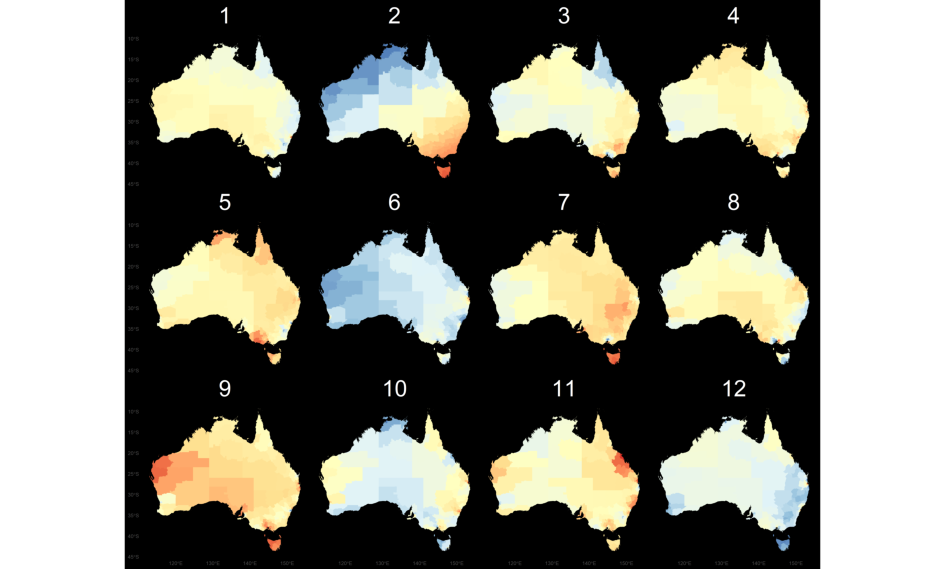
\includegraphics{thesis_files/figure-latex/nwse-hex2-1.pdf}
\caption{\label{fig:nwse-hex2}The lineup of hexagon tile map displays, location 12 contains a distribution that affects all capital nwse.}
\end{figure}

\hypertarget{replicate-2-2}{%
\subsection{Replicate 2}\label{replicate-2-2}}

\begin{figure}
\centering
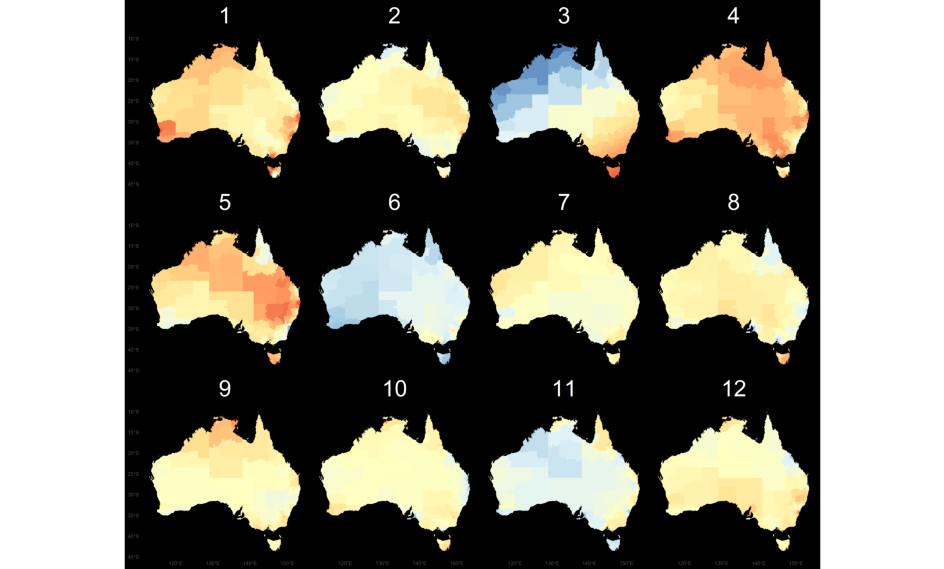
\includegraphics{thesis_files/figure-latex/nwse-geo3-1.pdf}
\caption{\label{fig:nwse-geo3}The lineup of choropleth map displays, location 3 contains a distribution that affects all capital nwse.}
\end{figure}

\begin{figure}
\centering
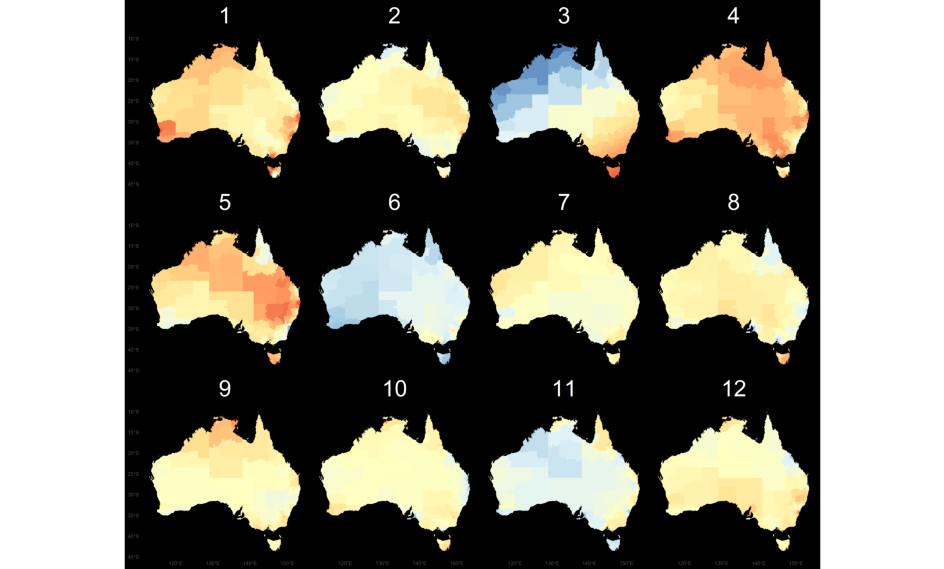
\includegraphics{thesis_files/figure-latex/nwse-hex3-1.pdf}
\caption{\label{fig:nwse-hex3}The lineup of hexagon tile map displays, location 3 contains a distribution that affects all capital nwse.}
\end{figure}

\hypertarget{replicate-3-2}{%
\subsection{Replicate 3}\label{replicate-3-2}}

\begin{figure}
\centering
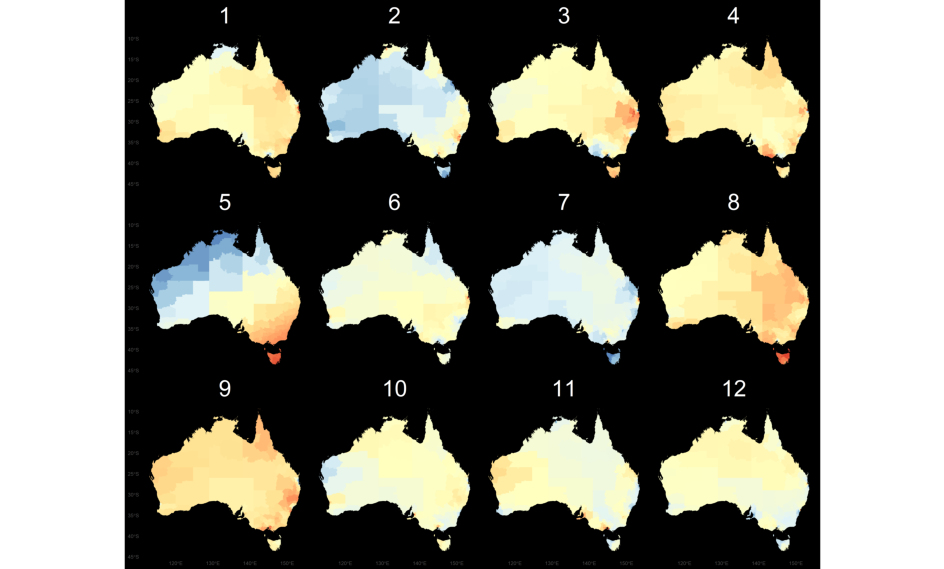
\includegraphics{thesis_files/figure-latex/nwse-geo5-1.pdf}
\caption{\label{fig:nwse-geo5}The lineup of choropleth map displays, location 4 contains a distribution that affects all capital nwse.}
\end{figure}

\begin{figure}
\centering
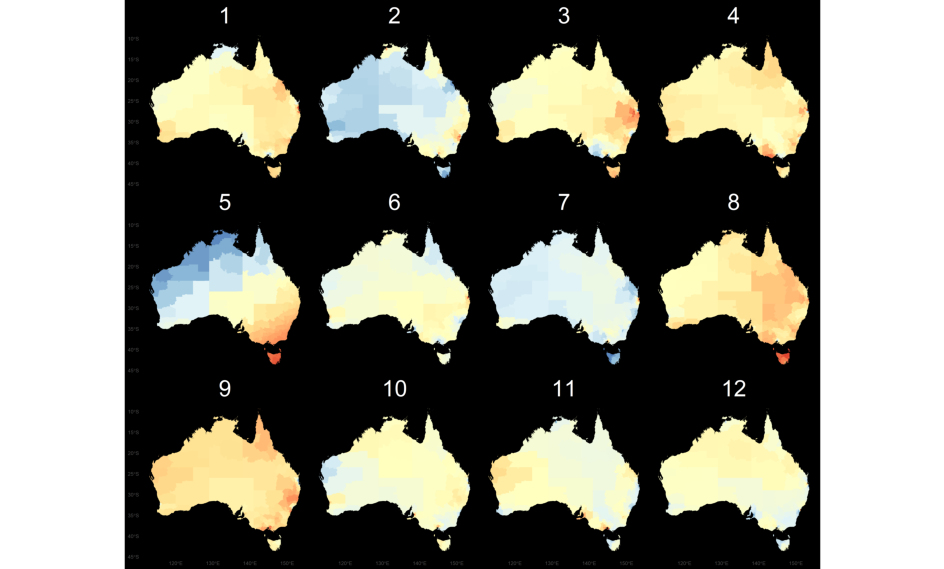
\includegraphics{thesis_files/figure-latex/nwse-hex5-1.pdf}
\caption{\label{fig:nwse-hex5}The lineup of hexagon tile map displays, location 4 contains a distribution that affects all capital nwse.}
\end{figure}

\hypertarget{replicate-4-2}{%
\subsection{Replicate 4}\label{replicate-4-2}}

\begin{figure}
\centering
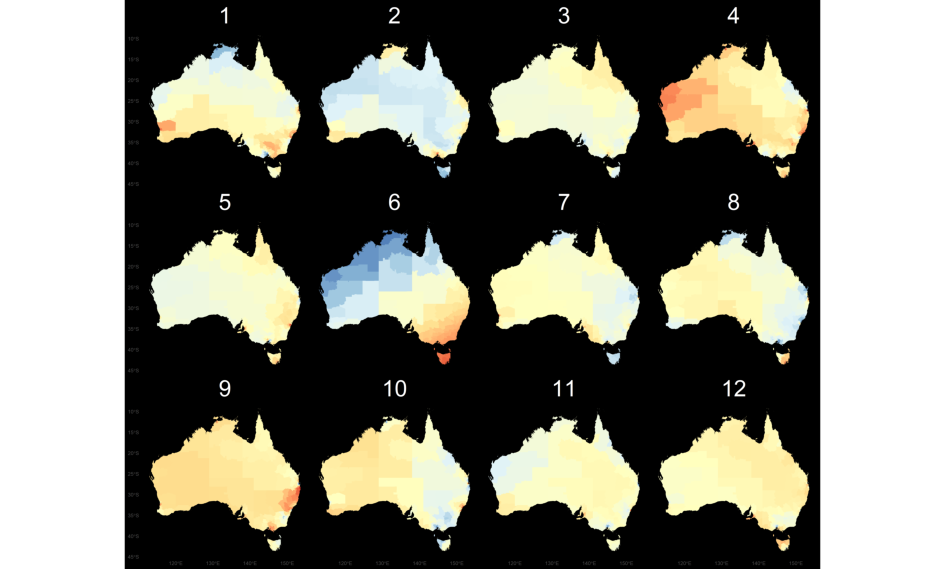
\includegraphics{thesis_files/figure-latex/nwse-geo6-1.pdf}
\caption{\label{fig:nwse-geo6}The lineup of choropleth map displays, location 9 contains a distribution that affects all capital nwse.}
\end{figure}

\begin{figure}
\centering
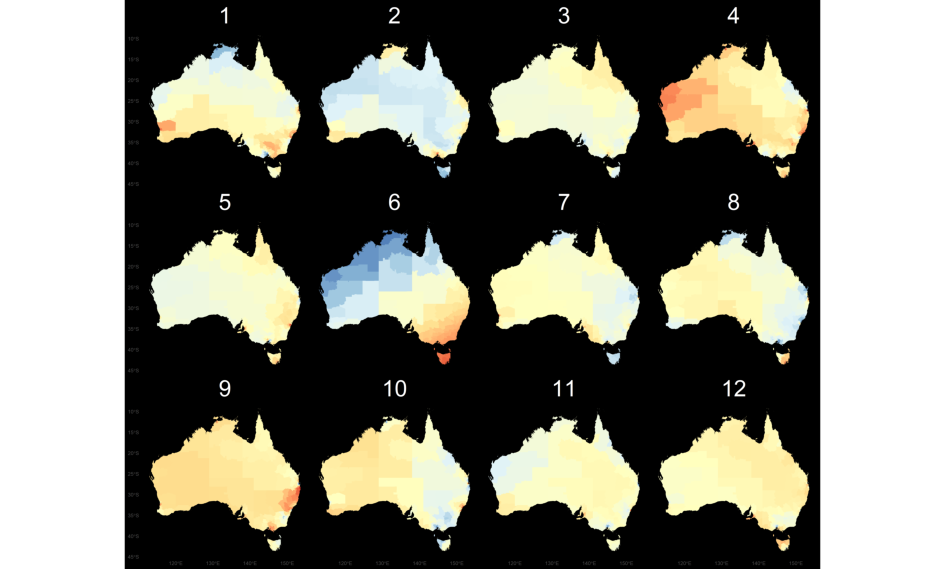
\includegraphics{thesis_files/figure-latex/nwse-hex6-1.pdf}
\caption{\label{fig:nwse-hex6}The lineup of hexagon tile map displays, location 9 contains a distribution that affects all capital nwse.}
\end{figure}

\hypertarget{visual-inference-study-survey-procedure}{%
\chapter{Visual inference study survey procedure}\label{visual-inference-study-survey-procedure}}

Participants were recruited via advertising on the Figure-Eight crowdsource platform.
Choosing the task from the list directed all potential participants to the page of instructions.
This page contained written instructions and is shown in Fig. \ref{fig:instruct}.

\begin{figure}
\centering
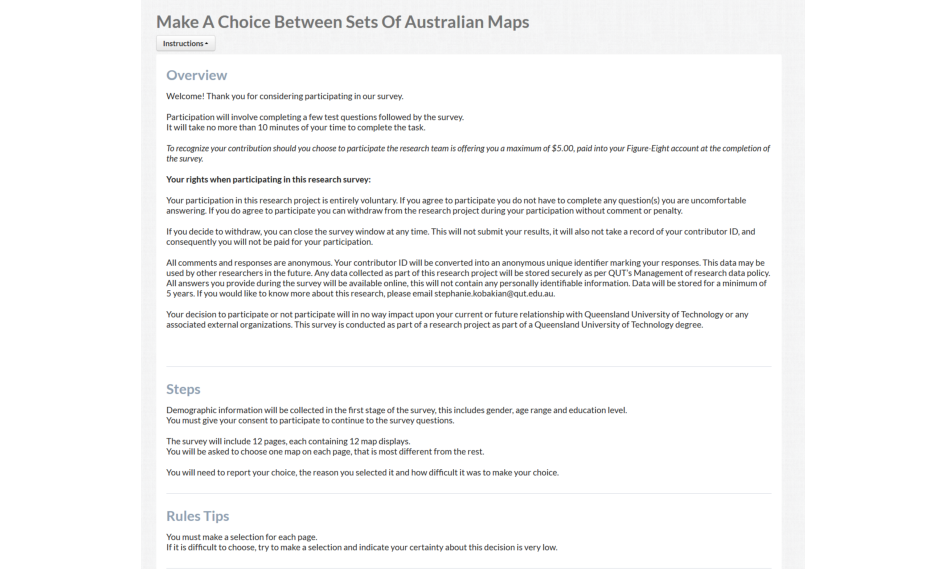
\includegraphics{thesis_files/figure-latex/instruct-1.pdf}
\caption{\label{fig:instruct}The training lineups of choropleth maps.}
\end{figure}

\hypertarget{training}{%
\section{Training}\label{training}}

The participants were trained using three displays. There were relatively simple lineups, they are displayed in Fig. \ref{fig:training1} and Fig. \ref{fig:training2}.

\begin{figure}
\centering
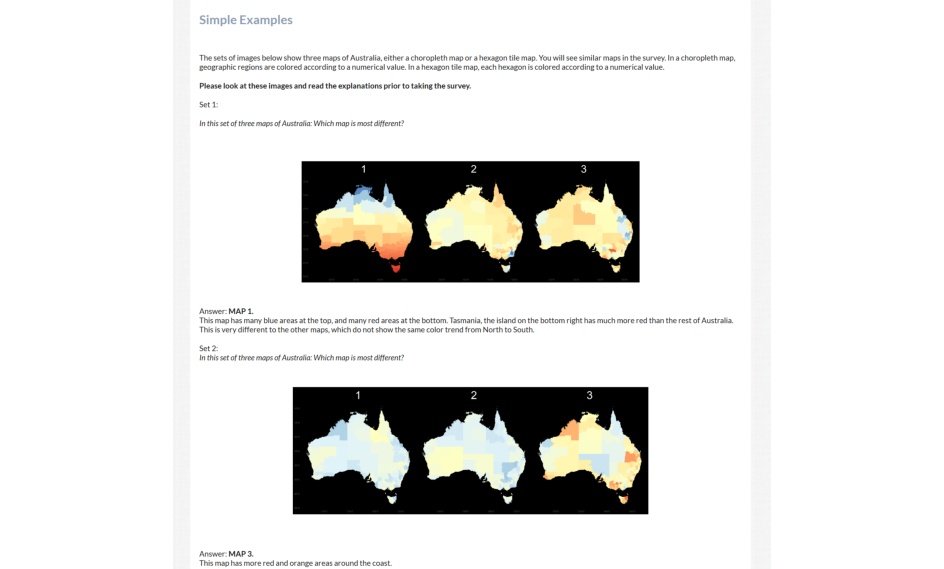
\includegraphics{thesis_files/figure-latex/training1-1.pdf}
\caption{\label{fig:training1}The training lineups of choropleth maps.}
\end{figure}

\begin{figure}
\centering
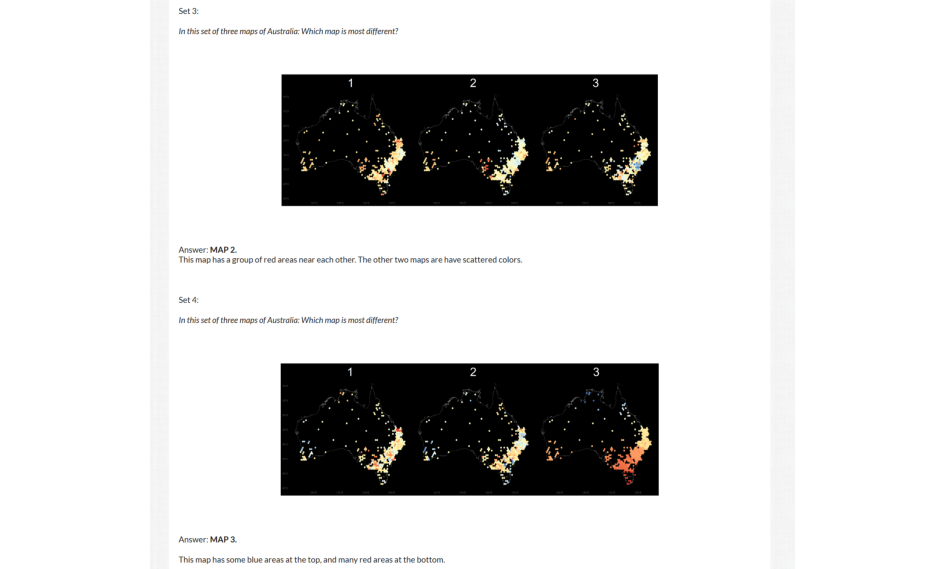
\includegraphics{thesis_files/figure-latex/training2-1.pdf}
\caption{\label{fig:training2}The training lineups of hexagon tile maps.}
\end{figure}

\hypertarget{survey-application}{%
\section{Survey application}\label{survey-application}}

The survey application was a \texttt{shinydashboard} we application, hosted on a website external to the Figure-Eight platform. The link to the survey was located at the bottom of the instructions and training page. Only participants who had read all of the instructions and seen the example image sets continued to the survey via the link.
This page also contained a question that asked participants for a validation code. The participants unique validation code was generated upon them opening the web application. This code was released to participants when they had considered all twelve lineups and submitted their responses to the \texttt{googlesheets} data set. Their validation codes were contained in the data set and associated with each of their responses.

The demographic and consent page of the \texttt{shinydashboard} web application are displayed in Fig. \ref{fig:survey-demogs}. Two example lineups are shown, one choropleth map lineup in Fig. \ref{fig:survey-choro} and one heaxgon tile map lineup in Fig. \ref{fig:survey-hex}.

\begin{figure}
\centering
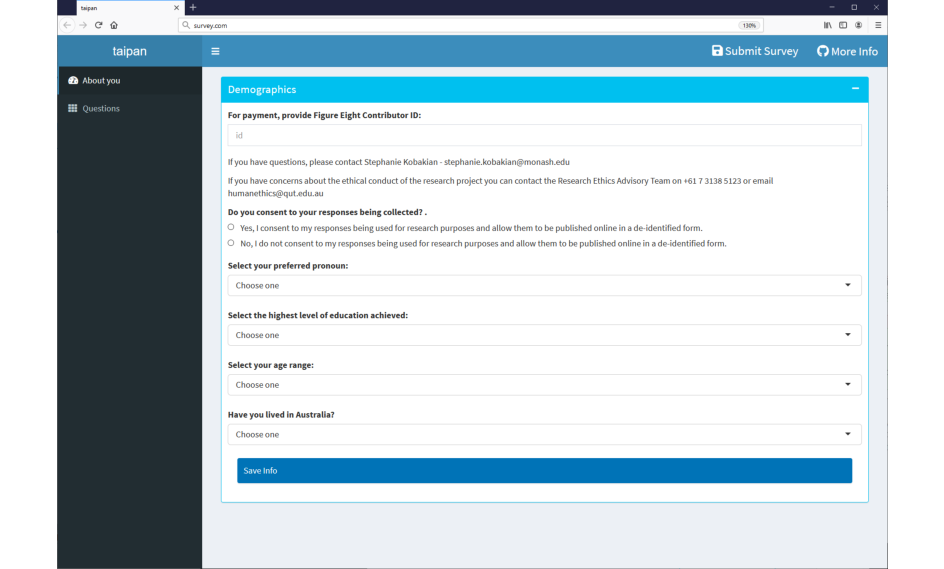
\includegraphics{thesis_files/figure-latex/survey-demogs-1.pdf}
\caption{\label{fig:survey-demogs}The demographics questions tab of the shinydashboard survey application.}
\end{figure}

\begin{figure}
\centering
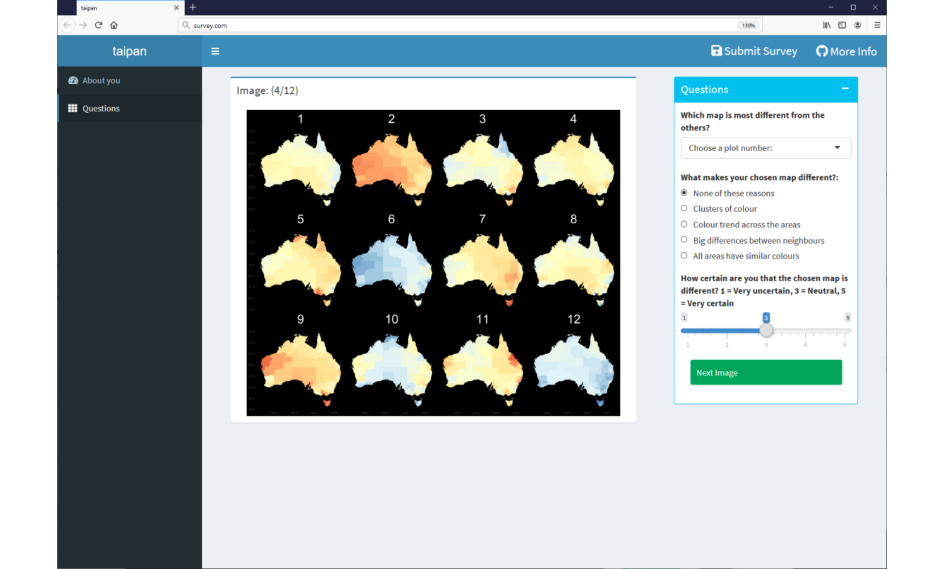
\includegraphics{thesis_files/figure-latex/survey-choro-1.pdf}
\caption{\label{fig:survey-choro}An example of the choropleth map lineup shown in the survey tab of the shinydashboard app.}
\end{figure}

\begin{figure}
\centering
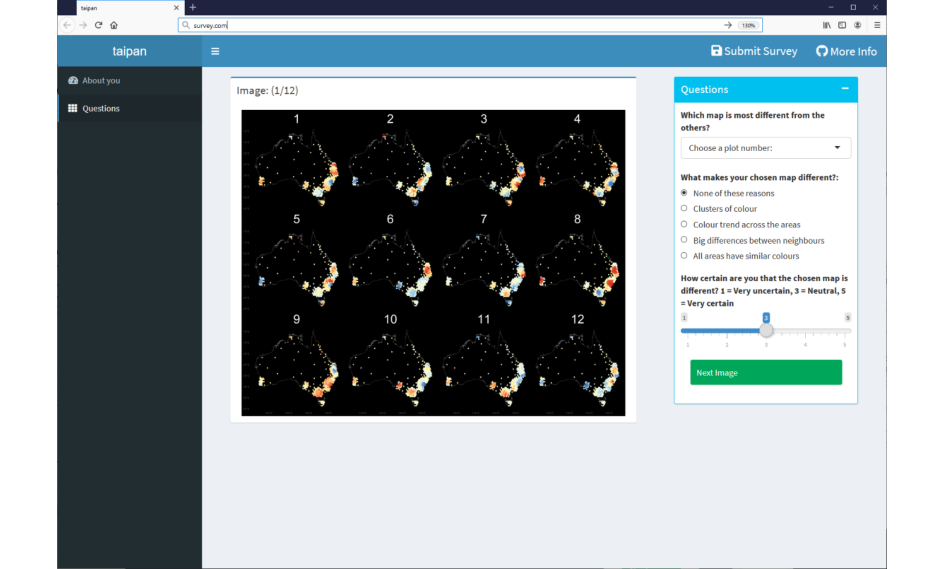
\includegraphics{thesis_files/figure-latex/survey-hex-1.pdf}
\caption{\label{fig:survey-hex}An example of the hexagon tile map lineup shown in the survey tab of the shinydashboard app.}
\end{figure}

\hypertarget{ch:ethics}{%
\chapter{Ethics Approval}\label{ch:ethics}}

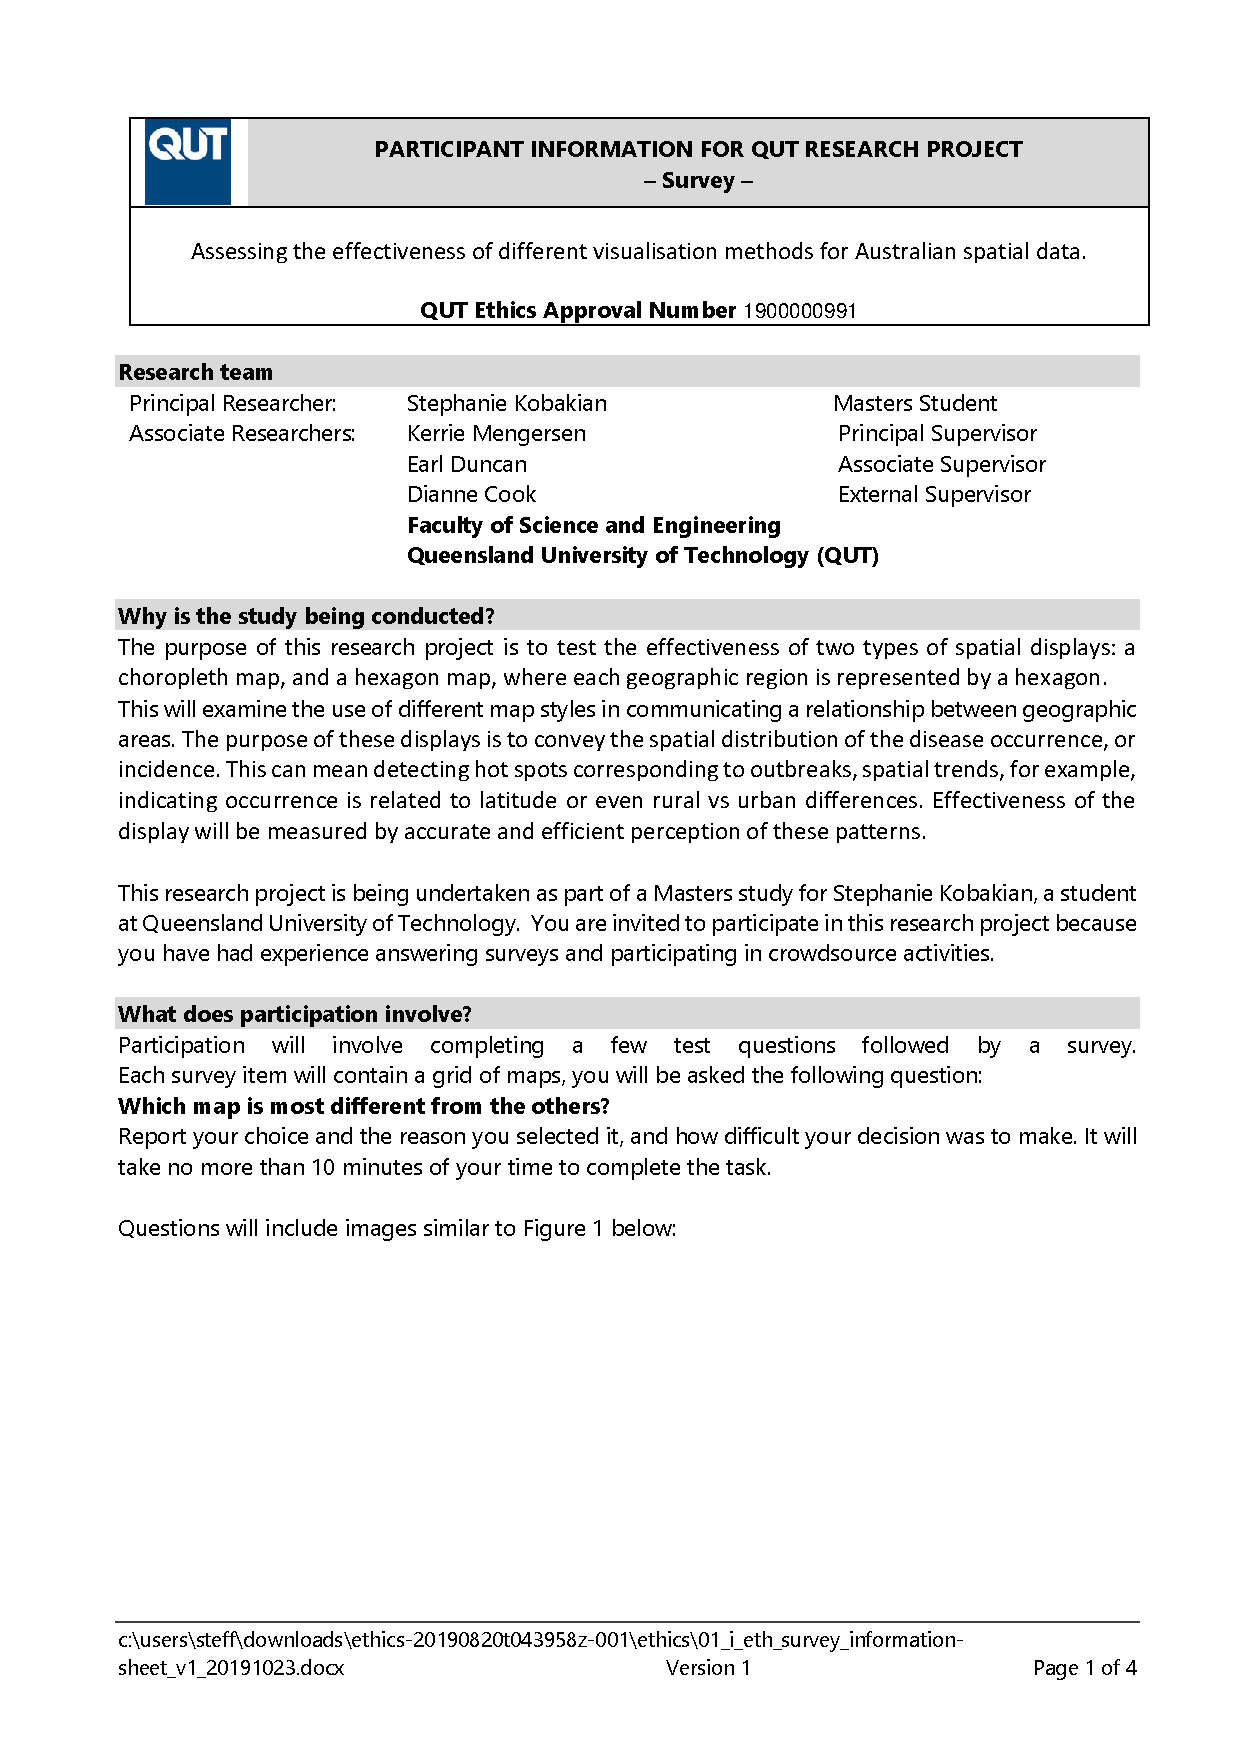
\includepdf[pages = {1-}, scale=1]{Ethics_1.pdf}

\printbibliography[heading=bibintoc]



\end{document}
